\chapter{Introduction}
\label{ch:introduction}

\note{Most of this chapter is probably going to be rewritten}

At present, ever larger sets of increasingly higher dimensional data are being produced, gathered and analyzed. As a consequence, several challenges arise when analyses are carried out on these vast amounts of high dimensional data. This recent surge of data prompts not only for the development of methods for data analysis capable of scaling to massive data sets but ones which are simultaneously capable of dealing with challenges inherent to high dimensional data.

In literature, problems arising from high dimensionality are collectively referred to as the \textit{curse of dimensionality}. Particularly in machine learning the following aspects of high dimensionality are problematic

\begin{itemize}
\item distances between pairs of points become less distinguished as dimensionality of the space increases \cite{on_the_surprising_behavior_of_distance_metrics}, rendering methods based on distance metrics at a disadvantage.
\item The volume of a space grows exponentially along with the number of dimensions. This leads to even large data sets appearing sparse in the feature space. Efficient sampling requires a lot of points
\item need for more training data, k-means example \cite[p.~263]{understanding_machine_learning}
\item algorithm complexity depends on the dimensionality of data being processed
\item from a more practical perspective, high dimensional data by itself is hard to directly reason about and difficult to visualize in any meaningful sense, as simple statistics will often not be able to capture adequate information of the data distribution.
\end{itemize}

The given listing is not exhaustive, but rather serves as an illustration for the variety of issues that can be encountered when working with high dimensional data.

To tackle problems associated with high dimensional data a common approach is to seek for a lower dimensional representation of the data which retains its salient features. This process, known as dimensionality reduction, can be split into two different approaches, namely \textit{feature selection} and \textit{feature extraction}.

The so-called manifold hypothesis \cite{manifold_hypothesis} often holds for real-world data sets. The manifold hypothesis posits that the high dimensional data in question lies near a much lower dimensional manifold. As an example, take ... . This in turn implies that if it is possible to learn this manifold, the original data could be described in far fewer dimensions with minimal loss of information. This, together with the classical Johnson-Lindenstrauss lemma \cite{johnson_lindenstrauss}, which provides general bounds to the error associated with dimensionality reduction between points of two Euclidean spaces, give a strong indication that for many data sets substantial dimensionality reduction is not only feasible, but that most of the information within the data can be captured with fewer parameters.

Several different methods for dimensionality reduction have been developed over the years. Arguably the most well known and applied dimensionality reduction method in practice is Principal Component Analysis (PCA), developed independently by Karl Pearson \cite{pca_1} and Harold Hotelling \cite{pca_2} in the early 1900s. Although very efficient to compute and providing easily interpretable results, PCA however suffers from the fact that it only takes into account linear relationships in the data it is given, making it nonideal for ... . The fact that PCA only aims to find an orthogonal projection that maximizes the variance... local structure of the data is poorly preserved. On the other hand, methods that aim to preserve local structure of data typically suffer from poor scalability to large data sets and the curse of dimensionality in several ways, such as ... .

\section{Scope and Objective}

As a wealth of dimensionality reduction methods have been developed, attempting to cover all of them would be greatly out of the scope of this thesis, in which the focus is on improving an existing method for primarily data visualization purposes. For comprehensive reviews on other prominent methods the reader is referred to \cite{first_dimensionality_reduction_review, second_dimensionality_reduction_review}.

In exploratory data analysis, visualization of the characteristics of data sets plays a key role. Being able to project high dimensional data into meaningful low dimensional representations enables researchers and data analysts to generate hypotheses.

In this work, a method for improving the applicability of parametric t-SNE is proposed. In the proposed method a generative model in the form of a Variational Autoencoder is first trained and subsequently used to produce training data for the parametric t-SNE embedding. The benefits of this procedure are severalfold: . Further, each of these benefits are experimentally demonstrated on a variety of data sets, both quantitatively and qualitatively.

\section{Outline}

The structure of this thesis is as follows. In Chapter~\ref{ch:background_and_related_work} the relevant background and related work to the contribution of this thesis is covered to give context to an audience not previously familiar with variational autoencoders or the t-SNE method for dimensionality reduction. The chapter is organized into two main sections, one that builds up to the theory and recent advances in variational autoencoders from the introduction of neural networks, and the other section presents the development of t-SNE up to its parametrization with neural networks.

The method developed for this thesis is presented in Chapter~\ref{ch:method}. The proposed learning and inference algorithms are presented, together with discussion on extensions and further variations. In addition, relevant implementation details of the application built to produce the results for the experiments chapter are briefly covered.

In Chapter~\ref{ch:experiments} the proposed method is tested experimentally for different properties presented in the previous chapter, as well as compared with existing methods. The experiments chapter includes descriptions for the various data sets being used and definitions for the metrics employed to quantitatively assess the quality of the produced low dimensional embeddings by our method and other methods under comparison.

The final chapter presents discussion and conclusions for the work carried out in this thesis. Additionally, directions for future work are suggested.

\chapter{Background and Related Work}
\label{ch:background_and_related_work}

\note{Some general background in more detail than the intro? Ideas listed below}

\begin{itemize}
\item main motivator for this work is to provide a tool to enhance exploratory analysis in cancer research
\item on molecular data
\item add references where visualization is used to aid analysis
\item discuss current state of the art
\item challenges associated with currently used methods
\item we outline in this chapter the relevant background information on the two methods that are used in the developed method, discussed in chapter \ref{ch:method}
\end{itemize}

\section{Variational Autoencoders}
\label{section:variational_autoencoders}

An essential component of the method presented in this work are Variational Autoencoders (VAE). VAEs belong to a broad class of models termed deep generative models, which have in recent years played an important role in machine learning research. As their name suggests, generative models attempt to model the process by which a given set of data has been generated by learning the underlying distribution of the data. Deep generative models are distinguished by the property that they are parameterized by neural networks, enabling the use of deep learning methods.

\note{short history of methods developed, RBM/DBN/DBM/GAN...} \cite{boltzmann_machines, deep_boltzmann_machines, deep_belief_nets, hinton_deep_belief_nets, gan}.

\note{Thorough review of deep generative models mentioned here, but which are out of scope for this work, can be found in \cite[Chapter~20]{deep_learning_book}.}

Before moving on to specialized artificial neural network structures and learning objectives, a brief review of the relevant background literature is presented. First, a general introduction to artificial neural networks is given, after which autoencoder neural networks are discussed in more detail. The theory and purpose of variational Bayesian methods are discussed to finally arrive at the full definition of VAEs by bringing together the contents of the preceding sections.

\subsection{Artificial Neural Networks}
\label{section:artificial_neural_networks}

Artificial neural networks, or as commonly referred to simply as neural networks, are a computational framework inspired by the biology of animal brains, more specifically the interconnected structure of individual nerve cells. Not unlike their biological counterparts, neural networks are composed of individual neurons capable of processing and passing along signals from one another to perform complex computation tasks as a whole.

Neural networks are at the core of many recent advances in machine learning. Particularly, deep neural network architectures now hold many state-of-the-art results in fields including computer vision, natural language processing, and speech recognition \cite{deep_learning}. More broadly, neural networks have been applied to all different categories of machine learning tasks, i.e. supervised, semi-supervised and unsupervised learning, with great success.

Advances in supervised learning for computer vision have arguably played an important role in the development of modern machine learning. A turning point for deep learning was the success of a deep convolution neural network architecture \cite{imagenet_alexnet}, later dubbed AlexNet, which performed considerably better than its competition in the 2012 ImageNet Large Scale Visual Recognition Challenge \cite{imagenet, imagenet_challenge}.

On the unsupervised learning front, deep belief networks, or rather unsupervised pretraining by stacking RBMs is one of the most important results in reviving interest in deep learning, as it was one of the first generally applicable results to enable learning of deep networks by means of better initialization of network parameters. More generally, learning meaningful representations from unlabeled data is an active research area, where methods of deep learning are producing state-of-the-art results with models such as the VAE, GAN and their variants.

Recently, deep learning in conjunction with reinforcement learning has produced superhuman results on tasks where previous methods of artificial intelligence have failed, such as playing video games \cite{deep_atari}, the game of go \cite{alphago} and shortly after, a fully unsupervised variant capable of generalizing to other games, convincingly beating previously developed chess and shogi engines \cite{alphazero, alphazero_generalized}.

The development of ever faster hardware for accelerating the computations needed for deep learning has played a pivotal role in the resurgence of research interest in neural networks. Originally built to accelerate the linear algebra operations required to produce 3D computer graphics, graphics programming units (GPU) offer immense parallel computing capabilities compared to traditional central processing units (CPU). With the advent of programming languages and APIs targeting GPUs, general-purpose computing on this specialized hardware has been made possible and has subsequently been taken advantage of in research and development of applications making use of neural networks. Recently, hardware specialized solely for use with deep learning has been developed \cite{tpu} and microarchitectures of modern GPUs have begun to incorporate specialized computing units for deep learning \cite{nvidia_tensor_core}, indicating a strong and growing interest towards deep learning in both academia and industry alike.

\subsubsection{Structure of Neural Networks}

Neural networks can be thought of as being large function compositions. Each neuron that is part of the network acts as a single function, taking as input the weighted output of other neurons connected to it and outputting the value of the neuron's \textit{activation function}. Neural networks can be classified into two main categories: feedforward and recurrent neural networks. Thinking of neurons and their connections in terms of graphs, where neurons represent vertices and edges represent the flow of data from one neuron to another, these two categories correspond to acyclic directed graphs and directed graphs that may contain cycles. In this work we will limit our focus to feedforward neural networks as the methods discussed do not make use of recurrent neural network structures.

As an example, Figure~\ref{fig:nn} depicts a feedforward neural network taking input vectors $\bx$ of length $3$ and outputting vectors $\mathbf{y}$ of length $2$.\footnote{Note that bias neurons have been omitted from the figure for simplicity.} The network can be seen to be split into three functionally distinct parts: an input layer, hidden layers, and an output layer. The input layer is directly fed the values to be run through the network. The hidden layers are formed by neurons connecting the input to the output layer. The output layer represents the result of the computation performed by the network. What this depicted neural network computes can be expressed with the equation

$$\mathbf{y} = f_3(\bW_3 f_2(\bW_2 f_1(\bW_1 \bx + \mathbf{b}_1) + \mathbf{b}_2) + \mathbf{b}_3),$$

where $f_i$ are the activation functions, $\bW_i$ the matrices of weights, and $\mathbf{b}_i$ the biases of the $i$th layer. The purpose of an activation function is to alter incoming signals to induce nonlinearity into the network as well as impose constraints on the values that flow through specific neurons, enabling the learning of more complex functions with desired properties. Bias neurons enable the shifting of activation function outputs. Weights of the network control the signal strengths from one neuron to the other.

\begin{figure}[!htb]
  \centering
  \resizebox{0.7\textwidth}{!}{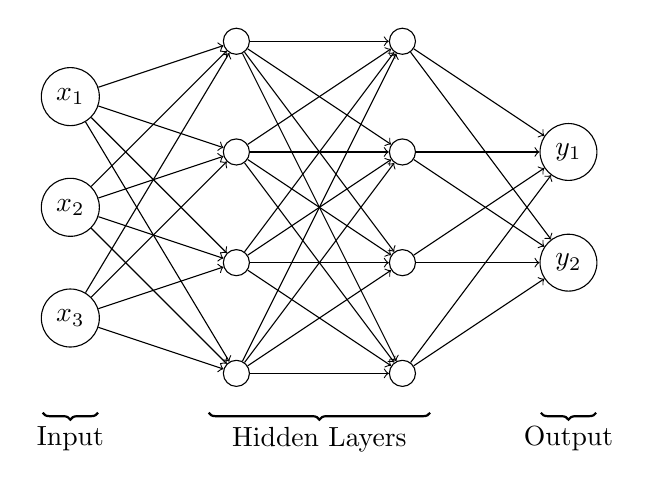
\begin{tikzpicture}[x=1em,y=1em]
  % Input layer
  \foreach \i in {1,...,3}{
    \node[draw, circle] (N-1-\i) at (0, 10 + 4 - 4 * \i) {$x_{\i}$};
  }
  % Hidden layer 1
  \foreach \i in {1,...,4}{
    \node[draw, circle] (N-2-\i) at (6, 12 + 4 - 4 * \i) {};
    \foreach \j in {1,...,3}{
      \draw [->] (N-1-\j) -- (N-2-\i);
    }
  }
  % Hidden layer 2
  \foreach \i in {1,...,4}{
    \node[draw, circle] (N-3-\i) at (12, 12 + 4 - 4 * \i) {};
    \foreach \j in {1,...,4}{
      \draw [->] (N-2-\j) -- (N-3-\i);
    }
  }
  % Output layer
  \foreach \i in {1,...,2}{
    \node[draw, circle] (N-4-\i) at (18, 8 + 4 - 4 * \i) {$y_{\i}$};
    \foreach \j in {1,...,4}{
      \draw [->] (N-3-\j) -- (N-4-\i);
    }
  }
\draw [thick, decoration={brace, mirror, raise=0.5cm}, decorate] (-1,0) -- (1,0) node[pos=0.5,anchor=north,yshift=-0.55cm] {Input};
\draw [thick, decoration={brace, mirror, raise=0.5cm}, decorate] (5,0) -- (13,0) node[pos=0.5,anchor=north,yshift=-0.55cm] {Hidden Layers};
\draw [thick, decoration={brace, mirror, raise=0.5cm}, decorate] (17,0) -- (19,0) node[pos=0.5,anchor=north,yshift=-0.55cm] {Output};
\end{tikzpicture}
\unskip}
  \caption{Feedforward neural network with input dimension 3, output dimension 2 and 2 hidden layers of dimension 4 each.}
  \label{fig:nn}
\end{figure}

\subsubsection{Learning in Neural Networks}

A simplistic view of neural networks would be to consider them merely as powerful function approximators. The theoretical underpinning for this view is the universal approximation theorem \cite{universal_approximation_theorem}, which states that under mild conditions on the activation function, neural networks with a single hidden layer can arbitrarily well approximate any continuous function.\footnote{The universal approximation theorem requires that the activation function is nonconstant, bounded and continuous, which highlights the importance of nonlinear activation functions.}$^{,}$\footnote{To be precise, this approximation applies to continuous functions defined on compact subsets of $\mathbb{R}^n$.} However, the universal approximation theorem does not state anything about the challenges associated with the learnability of the parameters for these approximations, which is where many of the practical challenges associated with neural networks lie.

Learning in neural networks boils down to the efficient finding of correct weights for the network to produce desired outputs for given inputs. How well a given network performs is evaluated by computing the value of its \textit{objective function}, given the knowledge of the input and output values. Finding weights for a given network thus becomes a problem of optimizing the value of its objective function. In this manner, neural networks can be trained for various computational tasks by choosing a suitable network architecture and specifying an objective function that models the computational task the network is desired to perform.

Early on in the development of neural networks the simple yet powerful backpropagation algorithm was developed independently by multiple researchers and later popularized by Rumelhart et al. \cite{nature_backprop} to enable the efficient training of neural networks. In essence, backpropagation is an algorithm to optimize neural network weights by exploiting their compositional structure and the chain rule of derivatives.

The backpropagation algorithm consists of two steps, the forward pass and the backward pass. In the forward pass input values are propagated through the network and the value of the objective function is computed. \tred{In the backward pass the gradient of the objective function is computed recursively w.r.t. all the weights of the network by beginning at the output layer and applying the chain rule to propagate the calculation back through the network. These gradients are then used to update the weights.}

Various optimization methods can be used in conjunction with the backpropagation algorithm to perform the weight updates w.r.t. the computed deltas. \note{On different optimization methods. SGD, gradient descent optimization methods (mention second order methods like \cite{kfac}?)}

\note{Is an example needed here or can we just defer the more concrete technicalities for the autoencoders chapter? Something along the lines of: As an example, and perhaps the most common task neural networks are applied to is statistical classification. The aim of classification is to assign observations to one of a set of predetermined categories. For instance, one might want to classify images of animals by species. The standard strategy for performing classification with neural networks is to construct a network whose input corresponds to a single observation being classified and the output layer having dimensions equal to the number of categories under consideration, where the activation function applied to the final layer is the softmax function. The purpose of the softmax activation is to have the output of the network correspond to the class assignment probabilities of each input, as it squashes the value of each output to the range $(0, 1)$ in a way that they sum to $1$. The objective...}

Several difficulties still arise when attempting to utilize neural networks, e.g. how to avoid poor local minima, how to converge faster, and how to avoid overfitting. In recent years, both theoretical and empirical work has been conducted to better understand these phenomena as well as develop methods to combat the difficulties they impose on learning in neural networks. \note{explain some of the recent research regarding convergence, vanishing gradients, adaptive momentum based methods, regularization, training deeper networks ... \cite{batch_normalization, dropout, relu, resnet}, and how there still isn't consensus on why some established methods seem to work (\cite{how_batch_norm_works}) (learning rate/batch size choice for optimization \cite{large_batch_size_generalization, learning_rate_vs_batch_size}) (potentially worse generalization of adaptive gradient methods, such as AdaGrad, RMSProp, Adam \cite{marginal_value_of_adaptive_gradient_methods}, even though empirical evidence suggests generally better performance on real-world data sets.)}

\begin{figure}[!htb]
  \centering
  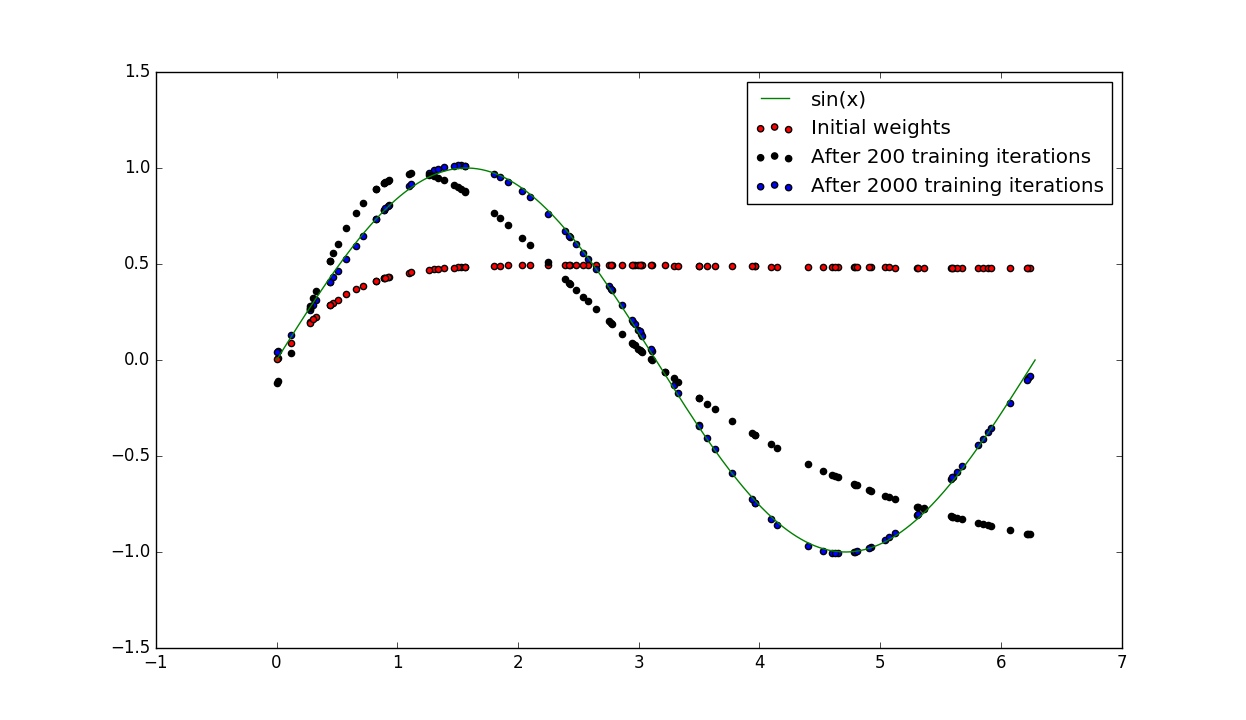
\includegraphics[width=0.8\textwidth]{images/function_approximation.png}
  \caption{Approximating a non-linear function with a neural network.}
  \label{fig:function_approximation}
\end{figure}

\subsection{Autoencoders}
\label{subsection:autoencoders}

First discussed in \cite{encoding_problem} as "the encoding problem", autoencoders (AE) are a class of neural network architectures designed for unsupervised representation learning. In essence, unsupervised representation learning attempts to find relevant features of a given data set without additional input to guide the process. Development of such methods is of interest to bypass the need for manual feature engineering.

The structure of autoencoders can be decomposed into two parts, namely the encoder and decoder. As the constituents' names suggest, part of the network performs encoding of the input and the other decoding of the encoded input, hence the name of this neural network architecture as a whole referring to "self-encoding". An example autoencoder network has been visualized in Figure~\ref{fig:ae}.

The learning objective of autoencoders is for the network to be able to reconstruct its inputs as faithfully as possible. A common objective function to train an autoencoder with is to have it minimize the mean squared error (MSE) between its input and output:

\begin{equation}
  \mathcal{L}_{MSE} = \frac{1}{N} \sum_{i=1}^{N} \norm{\bxi - \hat{\bx}^{(i)}}^2,
  \label{eq:mse}
\end{equation}

where $\bxi$ is the $i$th original input, $\hat{\bx}^{(i)}$ the reconstruction obtained by first encoding and then decoding the input and $N$ is the size of the data set. Through optimization of such reconstruction the network attempts to learn to produce an efficient encoding capable of capturing salient features of the data it has been trained on.

In a trivial case, where the network has too much capacity for modeling the input data, the AE can simply learn an identity mapping. This is clearly not conducive to learning meaningful latent representations of the data.

\tred{Case where the latent code's dimensionality is smaller than the original data's dimensionality. This \textit{bottleneck} potentially discards data, leading to a \textit{lossy compressed} representation.}

Autoencoders with multiple hidden layers were historically hard to optimize, as often gradient descent would get stuck in poor local minima. A method for initializing weights via stacking RBMs and fine-tuning with gradient descent first described in \cite{hinton_autoencoder} showed the efficacy of deep learning for non-linear dimensionality reduction.

A connection between PCA and autoencoders which are constrained to only have linear activation functions and are optimized with the MSE objective (see Equation~\ref{eq:mse}) has been shown in \cite{autoencoder_pca}. Additionally, it is shown that the optimization landscape of such an autoencoder is convex.

Even though autoencoders provide a powerful and scalable non-metric approach to dimensionality reduction there are a few disadvantages inherent to how they learn representations. \note{Elaborate the potential downsides of this approach (how to interpret the learned representation when nonlinearity is introduced? how does it generalize? Regularization as ad-hoc additions to the objective).} To address these issues we will instead be considering a stochastic extension of the autoencoding framework in the upcoming parts of this work.

\begin{figure}[!htb]
  \centering
  \resizebox{0.8\textwidth}{!}{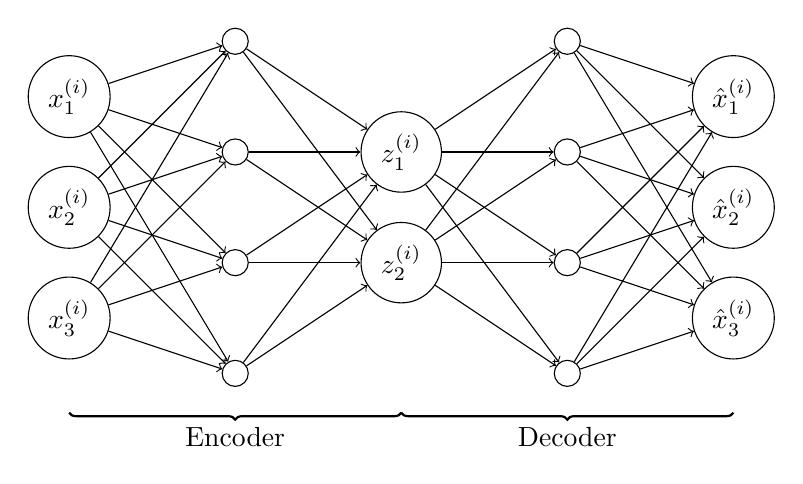
\begin{tikzpicture}[x=1em,y=1em]
  % Input layer
  \foreach \i in {1,...,3}{
    \node[draw, circle] (N-1-\i) at (0, 10 + 4 - 4 * \i) {$x^{(i)}_{\i}$};
  }
  % Encoder hidden layer
  \foreach \i in {1,...,4}{
    \node[draw, circle] (N-2-\i) at (6, 12 + 4 - 4 * \i) {};
    \foreach \j in {1,...,3}{
      \draw [->] (N-1-\j) -- (N-2-\i);
    }
  }
  % Latent code
  \foreach \i in {1,...,2}{
    \node[draw, circle] (N-3-\i) at (12, 8 + 4 - 4 * \i) {$z^{(i)}_{\i}$};
    \foreach \j in {1,...,4}{
      \draw [->] (N-2-\j) -- (N-3-\i);
    }
  }
  % Decoder hidden layer
  \foreach \i in {1,...,4}{
    \node[draw, circle] (N-4-\i) at (18, 12 + 4 - 4 * \i) {};
    \foreach \j in {1,...,2}{
      \draw [->] (N-3-\j) -- (N-4-\i);
    }
  }
  % Output layer
  \foreach \i in {1,...,3}{
    \node[draw, circle] (N-5-\i) at (24, 10 + 4 - 4 * \i) {$\hat{x}^{(i)}_{\i}$};
    \foreach \j in {1,...,4}{
      \draw [->] (N-4-\j) -- (N-5-\i);
    }
  }
\draw [thick, decoration={brace, mirror, raise=0.5cm}, decorate] (0,0) -- (12,0) node[pos=0.5,anchor=north,yshift=-0.55cm] {Encoder};
\draw [thick, decoration={brace, mirror, raise=0.5cm}, decorate] (12,0) -- (24,0) node[pos=0.5,anchor=north,yshift=-0.55cm] {Decoder};
\end{tikzpicture}
\unskip}
  \caption{Autoencoder with one hidden layer in both the encoder and decoder and latent dimensionality of 2.}
  \label{fig:ae}
\end{figure}

\subsection{Information Theory}

As a primer to variational inference, the main quantities of interest in information theory will be covered here, as they play a central role in all the subsequently discussed methods.

Information theory is the study of quantifying the information produced by a stochastic source.

\note{Start from definition of self-information}

$$I_{p(\bx)}(\bx) = -\log p(\bx)$$

The base of the logarithm determines the unit of information being considered, where popular choices are $2$ for bits and $e$ for nats. For convenience, we shall refer to bits as the unit of choice for the remainder of this section.

\note{Entropy, as the expectation of self-information of a stochastic source.}

$$H(p) = \mathbb{E}_{p(\bx)}[I_{p(\bx)}(\bx)] = \mathbb{E}_{p(\bx)}[-\log p(\bx)].$$

Using the formula defined above we can determine that the information entropy of a coin flip is $1$ bit, whereas the entropy of a 6-sided die roll is approximately $2.58$ bits.

\note{Give encoding interpretation of entropy and include cross-entropy defined as:}

$$H(p,q) = \mathbb{E}_{p(\bx)}[-\log q(\bx)]$$

Relative entropy, also known as the Kullback-Leibler divergence, or KL-divergence for short, ties together the concepts of entropy and cross-entropy. \note{Add the more practical explanation, which relates back to compression: $\dkl{p}{q}$ determines the average additional bits (or whichever unit is in use) needed for compression if $q$ is used as a surrogate for $p$.}

\note{define dkl in terms of entropy and cross entropy:}

$$\dkl{p}{q} = H(p,q) - H(p) = \mathbb{E}_{p(\bx)}[-\log \frac{q(\bx)}{p(\bx)}]$$

A second interpretation for KL-divergence is that of a measure of dissimilarity between two probability distributions. As such, \tred{...}

The following properties hold for KL-divergence:

\begin{enumerate}
\item $\dkl{p}{q} \geq 0$ (non-negativity)
\item $\dkl{p}{q} = 0 \iff p = q$ (identity of indiscernibles).
\end{enumerate}

One must note however that KL-divergence is asymmetric, i.e. $\dkl{p}{q} \neq \dkl{q}{p}$, and does not obey the triangle inequality, thus cannot readily be used as a metric. Especially asymmetry is important to take into account when interpreting the use of KL-divergence. Figure~\ref{fig:kl_divergence} visualizes the effect this asymmetry has as the KL-divergence between a Gaussian distribution $q$ and a mixture of Gaussians distribution $p$ is minimized.

\begin{figure}[!htb]
  \centering
  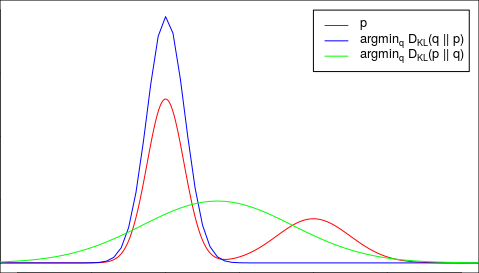
\includegraphics[width=0.7\textwidth]{images/kl_divergence.png}
  \caption{Asymmetry of KL-divergence as the KL-divergence between a Gaussian distribution $q$ and a mixture of Gaussians $p$ is minimized.}
  \label{fig:kl_divergence}
\end{figure}

\subsection{Variational Inference}
\label{subsection:variational_inference}

In modern statistics and machine learning a need to approximate highly complex probability distributions is a problem that often arises. A domain where such complex distributions are often encountered is Bayesian inference. The Bayes theorem states that the posterior distribution of latent variables conditioned on observed data is given by

$$p(\bz \vert \bx) = \frac{p(\bz, \bx)}{p(\bx)} = \frac{p(\bz, \bx)}{\int p(\bz, \bx) d\bz},$$

where the vector $\bx$ denotes the observed variables and $\bz$ the latent variables of the model. Even for only moderately complex models exact computation of the posterior is often intractable due to the required marginalization over all possible latent values $\bz$.

To illustrate this problem we will consider the same Bayesian mixture of Gaussians model described in \cite{variational_inference_review}. The model under consideration is univariate and consists of $K$ unit variance Gaussian mixture components. The full hierarchical model is given by the following

\begin{align*}
\mu_k                       &\sim \mathcal{N}(0, \sigma^2),                                     & k &= 1, \dotsc, K,\\
c_i                         &\sim \text{Categorical}(\nicefrac{1}{K}, \dotsc, \nicefrac{1}{K}), & i &= 1, \dotsc, n,\\
x_i \vert c_i, \bmu &\sim \mathcal{N}(c^{\top}_i \bmu, 1),                      & i &= 1, \dotsc, n,
\end{align*}

where each of the $n$ observations $x_i$ are generated by drawing the means of the $K$ Gaussian mixture components $\mu_k$ and the mixture component assignments $c_i$.\footnote{Note that $c_i$ is being encoded as an indicator $K$-vector, where all entries are zero except for the index that corresponds to the drawn categorical variable being $1$.} In this model the latent variables are $\bz = {\bmu, \mathbf{c}}$. From these definitions, the joint distribution factorizes as

$$p(\bmu, \mathbf{c}, \bx) = p(\bmu) \prod_{i=1}^{n} p(c_i) p(x_i \vert c_i, \bmu).$$

Now, when marginalizing out $\bmu$ and $\mathbf{c}$, we arrive at the following integral

$$p(\bx) = \int p(\bmu) \prod_{i=1}^{n} \sum_{c_i} p(c_i) p(x_i \vert c_i, \bmu) d\bmu.$$

As the time complexity of evaluating this integral is $\mathcal{O}(K^n)$, it is evident that direct computation quickly becomes infeasible even for relatively small $K$ and $n$.

The dominant paradigm for obtaining approximates for such distributions has been through various methods of sampling, such as Markov chain Monte Carlo (MCMC) methods like Gibbs sampling or the Metropolis-Hastings algorithm. \note{These sampling methods provide asymptotic guarantees of exactness. More computationally demanding but more accurate approximates than VI. VI more suited to the large data sets prevalent in modern machine learning.}

Variational inference takes a different approach to approximating the posterior. Instead of sampling, in variational inference the approximation problem is turned into an optimization problem. By considering a family of distributions $\mathcal{Q}$ one seeks to optimize

\begin{equation}
q^{*}(\bz) = \argmin_{q(\bz) \in \mathcal{Q}} \dkl{q(\bz)}{p(\bz \vert \bx)},
\label{eq:vi}
\end{equation}

where the quantity being optimized is the KL-divergence introduced in the previous section. The optimization tries to find a member $q^{*}(\bz)$ of the chosen family of distributions that best matches the true posterior, which can then be used as a surrogate for the true posterior.

In practice, the considered family of distributions $\mathcal{Q}$ is constrained in a way as to make optimization tractable. A common constraint is to assume the distributions of the chosen family factorize as follows

$$q(\bz) = \prod_{i=1}^{d} q_{i}(z_{i}),$$

which is referred to as the \textit{mean field approximation} in literature. The mean field approximation essentially removes from consideration all covariate structure as each variable of $\bz$ is considered independent. In the Gaussian case this means instead of optimizing $d^2$ variables of the covariance matrix we can instead limit optimization to only consider $d$ elements of a diagonal covariance matrix. An illustration of this for the case of two Gaussian distributions is presented in Figure~\ref{fig:mean_field_approximation}.

Seeing that Equation~\ref{eq:vi} cannot be directly optimized as it depends on evaluation of the intractable posterior, in variational inference one seeks to instead optimize an alternative objective that is tractable. To derive this alternative objective, we begin with the definition

\begin{equation}
\begin{aligned}
\dkl{q(\bz)}{p(\bz \vert \bx)} &= \mathbb{E}[\log \frac{q(\bz)}{p(\bz \vert \bx)}] \\
                               &= \mathbb{E}[\log q(\bz)] - \mathbb{E}[\log p(\bz \vert \bx)] \\
                               &= \mathbb{E}[\log q(\bz)] - \mathbb{E}[\log p(\bz, \bx)] + \log p(\bx),
\end{aligned}
\end{equation}

and by rearranging, it follows from the non-negativity property of KL-divergence that

\begin{equation}
\begin{aligned}
\log p(\bx) &= \dkl{q(\bz)}{p(\bz \vert \bx)} - \mathbb{E}[\log q(\bz)] + \mathbb{E}[\log p(\bz, \bx)] \\
            &= \underbrace{\dkl{q(\bz)}{p(\bz \vert \bx)}}_{\geq 0} + \mathbb{E}[\log p(\bx \vert \bz)] - \dkl{q(\bz)}{p(\bz)} \\
            &\geq \underbrace{\mathbb{E}[\log p(\bx \vert \bz)] - \dkl{q(\bz)}{p(\bz)}}_{\text{ELBO}}.
\end{aligned}
\end{equation}

This bound is better known as the \textit{evidence lower bound}, or ELBO for short. By maximizing this bound the optimization indirectly minimizes the KL-divergence between $q(\bz)$ and $p(\bz \vert \bx)$, which corresponds to the original objective of variational inference.

\note{It is possible to combine automatic differentiation with variational inference to further ease statistical model building and computational efficiency \cite{advi}. (Brief discussion on probabilistic programming)}

\begin{figure}[!htb]
  \centering
  \resizebox{0.5\textwidth}{!}{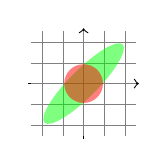
\begin{tikzpicture}[x=1em,y=1em]
\draw[->] (-2,0) -- (2,0) coordinate (x axis);
\draw[->] (0,-2) -- (0,2) coordinate (y axis);
\draw[step=0.75,gray,very thin] (-1.9,-1.9) grid (1.9, 1.9);
\fill[green, fill opacity=0.5, rotate around={45:(0,0)}, very thick] (0,0) ellipse (2.0 and 0.5);
\fill[red, fill opacity=0.5, very thick] (0,0) circle (0.7);
%\draw[very thick, green, opacity=0.5] (2, -2.0) -- node {Exact} (2,-1.9);
%\draw[very thick, red, opacity=0.5] (2, -1.85) -- node {Approximate} (2,-1.75);
\end{tikzpicture}
\unskip}
  \caption{Illustration of the mean-field approximation of a full rank Gaussian. Adapted from \cite{variational_inference_review}, Figure 1.}
  \label{fig:mean_field_approximation}
\end{figure}

\subsection{Autoencoding Variational Bayes}

VAEs extend autoencoders into probabilistic generative models. Instead of the deterministic encoding and decoding networks of traditional autoencoders, VAE encoders and decoders parameterize probability distributions. The encoder network parameterizes the distribution of the latent variable $\bz$ conditioned on its data $\bx$, whereas the decoder parameterizes the data distribution conditioned on a latent variable.

\note{Explain the relationship between latent variables, their distributions and why variational bayes is needed here. ... In terms of probability distributions the generative model $\ptheta(\bz) \ptheta(\bx \vert \bz)$ is parameterized by $\btheta$.}

To summarize, Figure~\ref{fig:aevb_plate_notation} depicts the graphical model under consideration, where $\bphi$ and $\btheta$ are the parameters of the encoder and decoder, respectively.

\begin{figure}[!htb]
  \centering
  \resizebox{0.3\textwidth}{!}{\begin{tikzpicture}
  \node[obs]                (x) {$\bx$};
  \node[latent, left=of x]  (z) {$\bz$};
  \node[latent, above=of x] (t) {$\btheta$};
  \node[latent, above=of z] (p) {$\bphi$};
  
  \edge[bend left]          {z} {x};
  \edge[bend left, dashed]  {x} {z};
  \edge                     {t} {z};
  \edge                     {t} {x};
  \edge[dashed]             {p} {z};
  
  \plate {zx} {(x)(z)}      {$N$};
\end{tikzpicture}
\unskip}
  \caption{The VAE graphical model, in plate notation. Adapted from \cite{aevb}, Figure 1.}
  \label{fig:aevb_plate_notation}
\end{figure}

\subsubsection{Derivation of the VAE Objective Function}

\note{TODO: Now there's overlap here with the VI section. Reword this as an example of it, rather than introducing the whole concept of ELBO again.}

The objective of VAEs is to model the generative process of a given data set as well as possible. The objective is derived from the maximization of the marginal likelihood $\ptheta(\bxi)$ of each data point $i$ in the given data set. By application of Jensen's inequality we can derive the following lower bound for the marginal likelihood for our latent variable model:

\begin{equation}
\begin{aligned}
\log \ptheta(\bxi) & = \log \int \ptheta(\bxi \vert \bz) \ptheta(\bz) d\bz \\
                   & = \log \int \frac{\qphi(\bz \vert \bxi)}{\qphi(\bz \vert \bxi)} \ptheta(\bxi \vert \bz) \ptheta(\bz) d\bz \\
                   & = \log \mathbb{E}_{\qphi(\bz \vert \bxi)}\Big[\frac{\ptheta(\bxi \vert \bz) \ptheta(\bz)}{\qphi(\bz \vert \bxi)}\Big] \\
                   & \geq \mathbb{E}_{\qphi(\bz \vert \bxi)}\Big[\log \frac{\ptheta(\bz)}{\qphi(\bz \vert \bxi)}\Big] + \mathbb{E}_{\qphi(\bz \vert \bxi)}\Big[\log \ptheta(\bxi \vert \bz)\Big] \\
                   & = -\dkl{\qphi(\bz \vert \bxi)}{\ptheta(\bz)} + \mathbb{E}_{\qphi(\bz \vert \bxi)}\Big[\log \ptheta(\bxi \vert \bz)\Big].
\end{aligned}
\end{equation}

This bound is better known as the \textit{evidence lower bound}, or ELBO for short, which we will denote as $\mathcal{L}(\btheta, \bphi; \bxi)$. An interpretation for the terms of the last equation is that the objective is to have the posterior $\qphi(\bz \vert \bxi)$ match the prior $\ptheta(\bz)$ as accurately as possible, acting as a regularizer, while simultaneously maximizing the expectation of the likelihood of $\bxi$ under the learnt latent distribution, i.e. having the decoder parameterize a distribution from which a draw of $\bxi$ is as likely as possible.

Several modifications to this objective have been proposed, e.g. the $\beta$-VAE \cite{beta_vae, understanding_beta_vae}, $\beta$-TCVAE \cite{beta_tcvae} and InfoVAE \cite{infovae}, which aim to improve the learning of better latent representations. Beta-VAE prefixes the KL term with a constant $\beta$ which is interpreted as a Lagrange multiplier that adjusts the regularization imposed by the latent prior. The case where $\beta = 1$ corresponds to the VAE formulation presented in this section, while $\beta > 1$ \note{more learning pressure to match the prior, for factorized models this corresponds to more "disentanglement". $\beta$-TCVAE decomposes the $\beta$-VAE loss for factorized models to reveal a correlation term between latent variables which it attempts to penalize. InfoVAE on the other hand attempts to maximize the mutual information between the latent code and the reconstructed output to enforce utilization of the latent code even when flexible decoder distributions are used.}

\subsubsection{Obtaining Differentiable Monte Carlo Estimates}

To optimize the parameters $\btheta$ and $\bphi$ of our neural network using backpropagation we require a way to compute the gradient of the expectations of random variables. The \textit{reparameterization trick} enables keeping all computation the neural network performs fully deterministic while still permitting the sampling of probability distributions parameterized by the network itself. By keeping all computation deterministic, backpropagation can be used to optimize the network.

\tred{The reparameterization trick works by introducing an auxiliary noise variable as input to the network and a suitable differentiable function is used to transform the input noise into a sample of the distribution parameterized by the neural network and the original input data. As in \cite{aevb}, we shall denote this function by $g_{\bphi}$, the latent variable samples are then obtained by}

$$\bz^{(i,l)} = g_{\bphi}(\bxi, \eil), \quad \eil \sim p(\beps).$$

The choice of distribution from which $\eil$ is drawn from and the analytic form of $g_{\bphi}$ depends on the distribution that is being reparameterized. \tred{For location-scale distributions ...}

$$\mathbb{E}_{\qphi(\bz \vert \bxi)}[f(\bz)] \simeq \frac{1}{L} \sum_{l=1}^{L} f(g_{\bphi}(\bxi, \eil))$$

\begin{equation}
\mathcal{L}(\btheta, \bphi; \bxi) = -\dkl{\qphi(\bz \vert \bxi)}{\ptheta(\bz)} + \frac{1}{L} \sum_{l=1}^{L} \log \ptheta(\bxi \vert \bz^{(i,l)})
\label{eq:vae_loss}
\end{equation}

In many cases the KL-divergence can be integrated analytically, for instance in the case of two Gaussian distributions. In cases where the KL term cannot be solved analytically a Monte Carlo estimate for the KL-divergence can be used:

\begin{equation}
\mathcal{L}(\btheta, \bphi; \bxi) = \frac{1}{L} \sum_{l=1}^{L} \Big[\qphi(\bz^{(i,l)} \vert \bxi) - p(\bz^{(i,l)}) + \log \ptheta(\bxi \vert \bz^{(i,l)})\Big].
\label{eq:vae_loss_2}
\end{equation}

\note{Should mention inability to reparameterize discrete distributions. A method for obtaining samples of a categorical distribution by relaxation to a continuous distribution \cite{gumbel_softmax}, can avoid marginalizing over all possible values of latent categorical variables in models like the M2 VAE.}
\tred{A drawback of the reparameterization trick is that it is only applicable to continuous distributions...}

\subsubsection{Network Structure}

Figure~\ref{fig:vae} depicts the network structure of a VAE whose encoder outputs the mean and standard deviation parameters of a distribution. These parameters could for instance be used to model the approximate posterior $\qphi(\bz \vert \bxi)$ as the multivariate Gaussian distribution $\mathcal{N}(\bmu^{(i)}, \bsigma^{(i)} \mathbf{I})$, where, with slight abuse of notation, $\bsigma^{(i)} \mathbf{I}$ stands for a diagonal covariance matrix whose diagonal is made up of the elements of the vector $\bsigma^{(i)}$.

It is important to note that the output $\hat{\bx}^{(i,l)}$ of the network in the figure should not be interpreted as the final reconstruction of the input like in traditional autoencoders, but rather as the values parameterizing the distribution $\ptheta(\bx \vert \bz^{(i, l)})$. For binary data, the distribution $\ptheta(\bx \vert \bz^{(i, l)})$ is commonly chosen to be a multivariate Bernoulli, where the decoder outputs $\hat{\bx}^{(i,l)}$ parameterize individual Bernoulli distributions, whereas for continuous data the parameters for a Gaussian distribution are typically outputted.

\note{Problem with variational inference, also apparent in our Gaussian encoder example here, is the inflexibility of the chosen distribution. Normalizing flows attempt to resolve this issue \cite{normalizing_flows, inverse_autoregressive_flow, householder_flow}, result in overall better $p(\bx)$, and with VAE these flows can be learned efficiently.}

\note{Extensions to semi supervised and adversarial learning \cite{semi_supervised_vae, adversarial_autoencoders}.}

\begin{figure}[!htb]
  \centering
  \resizebox{0.8\textwidth}{!}{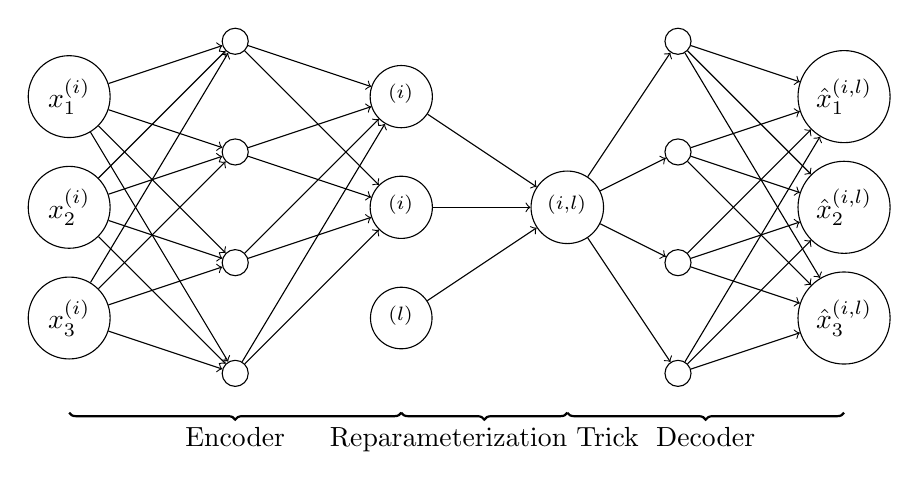
\begin{tikzpicture}[x=1em,y=1em]
  % Input layer
  \foreach \i in {1,...,3}{
    \node[draw, circle] (N-1-\i) at (0, 10 + 4 - 4 * \i) {$x^{(i)}_{\i}$};
  }
  % Encoder hidden layer
  \foreach \i in {1,...,4}{
    \node[draw, circle] (N-2-\i) at (6, 12 + 4 - 4 * \i) {};
    \foreach \j in {1,...,3}{
      \draw [->] (N-1-\j) -- (N-2-\i);
    }
  }
  % Latent code
  \node[draw, circle] (mu) at (12, 10) {$\bmu^{(i)}$};
  \node[draw, circle] (sigma) at (12, 6) {$\bsigma^{(i)}$};
  \node[draw, circle] (eps) at (12, 2) {$\beps^{(l)}$};
  \node[draw, circle] (z) at (18, 6) {$\bz^{(i, l)}$};
  \foreach \x in {mu,sigma,eps}{
    \draw [->] (\x) -- (z);
  }
  \foreach \x in {mu,sigma}{
    \foreach \j in {1,...,4}{
      \draw [->] (N-2-\j) -- (\x);
    }
  }
  % Decoder hidden layer
  \foreach \i in {1,...,4}{
    \node[draw, circle] (N-4-\i) at (22, 12 + 4 - 4 * \i) {};
    \draw [->] (z) -- (N-4-\i);
  }
  % Output layer
  \foreach \i in {1,...,3}{
    \node[draw, circle] (N-5-\i) at (28, 10 + 4 - 4 * \i) {$\hat{x}^{(i, l)}_{\i}$};
    \foreach \j in {1,...,4}{
      \draw [->] (N-4-\j) -- (N-5-\i);
    }
  }
  \draw [thick, decoration={brace, mirror, raise=0.5cm}, decorate] (0,0) -- (12,0) node[pos=0.5,anchor=north,yshift=-0.55cm] {Encoder};
  \draw [thick, decoration={brace, mirror, raise=0.5cm}, decorate] (12,0) -- (18,0) node[pos=0.5,anchor=north,yshift=-0.55cm] {Reparameterization Trick};
  \draw [thick, decoration={brace, mirror, raise=0.5cm}, decorate] (18,0) -- (28,0) node[pos=0.5,anchor=north,yshift=-0.55cm] {Decoder};
\end{tikzpicture}
\unskip}
  \caption{Variational Autoencoder. Note that the hidden layer values $\bmu^{(i)}$, $\bsigma^{(i)}$ and the input noise variable $\beps^{(l)}$ represent vectors instead of single values for a cleaner visual representation.}
  \label{fig:vae}
\end{figure}

\section{t-Distributed Stochastic Neighbor Embedding}
\label{section:tsne}

Taking a slight departure from the preceding discussion on neural networks, the theory, and development leading to the acclaimed dimensionality reduction algorithm t-SNE will be presented. At the end of this section, a way to utilize the t-SNE objective to train an embedding function parameterized by a neural network will be shown, thereby connecting this section with the previous in a natural way, as well as covering the final preliminaries to the contribution of this thesis.

\subsection{SNE}
\label{subsection:sne}

The Stochastic Neighbor Embedding (SNE) algorithm \cite{sne}, developed by Hinton and Roweis in 2003, serves as the precursor to the later improved t-SNE algorithm. As such, SNE shares many similarities in its definition with t-SNE, and thus by first developing an understanding of SNE and its pitfalls the motivation behind the t-SNE algorithm become more apparent.

As the algorithm's name suggests, the approach SNE takes to perform dimensionality reduction is probabilistic in nature. Without delving directly into the mathematical details, an intuitive overview of the algorithm is that it attempts to embed data points in a lower dimension by preserving probability distributions defined on the pairwise distances of points. More concretely, the algorithm proceeds as follows. First, for all data points probability distributions for how likely it is to pick each point as its neighbor in both input and output space are formed. After these probability distributions have been formed, the actual embedding is performed by attempting to distribute the points in the output space such that similarly defined probability distributions in the output space match those of the input space as closely as possible. The natural way to match two distributions is familiar from the discussion on variational bayes methods, namely the KL-divergence between the input and output space distributions is used as the objective function for the embedding of data points, which can be optimized with various methods, including the previously covered gradient descent.

To formalize these notions, we begin with how the conditional probability of data point $i$ picking data point $j$ in the input space is defined by the equation

\begin{equation}
p_{j \vert i} = \frac{exp(-\norm{\bx_i - \bx_j}^2 / 2 \sigma_i^2)}{\sum_{k \neq i} exp(-\norm{\bx_i - \bx_k}^2 / 2 \sigma_i^2)},
\label{eq:p_j_c_i}
\end{equation}

where the probability can be seen as being derived as if a Gaussian were centered on $\bx_i$ and an appropriate normalizing term is used to scale the individual probabilities so that they sum to $1$. The variance (denoted by $\sigma_i$ in the equation) is determined separately for each data point $i$ by forcing the perplexity of the conditional distribution over all other data points (later denoted as $P_i$) to equal some preset value.

Perplexity is an information theoretic measure of how well a distribution predicts its samples. For a given probability distribution, perplexity is defined as the exponentiation of the distribution's entropy $H$, e.g. in the case of our discrete $P_i$:

$$b^{H(P_i)} = b^{-\sum_{j=1}^{n} p_{j \vert i} \log_b p_{j \vert i}},$$

where $b$ is the unit used to measure entropy, typically chosen to be either $2$ or $e$, for bits or nats, respectively. From the definition, we can see that larger variance will be chosen for the Gaussians in areas of the input space where the density of data points is low and smaller variance will be used in high density areas. Effectively, variance is adapted to fit the core assumption that the data points lie on a uniformly sampled manifold within the input space. Perplexity is thus a value proportional to the number of effective local neighbors considered by the algorithm when the embedding is being optimized. In practice, the correct $\sigma_i$ for each $i$ is numerically sought using the bisection method, up to a small error tolerance in the resulting perplexity.

The conditional distribution in the output space is similarly defined with a Gaussian kernel:

$$q_{j \vert i} = \frac{exp(-\norm{\mathbf{y}_i - \mathbf{y}_j}^2)}{\sum_{k \neq i} exp(-\norm{\mathbf{y}_i - \mathbf{y}_k}^2)},$$

where each $\mathbf{y}_i$ represents the point in the embedding for data point $\bx_i$. A notable difference is the absence of the variance term $2 \sigma_i^2$, which can be interpreted as having been set to $1$ throughout. This choice of fixed variance can, in turn, be interpreted as smoothing out the manifold of the input space when performing the embedding.

Now that we have defined both the output and input distributions for points, the objective function can be formulated as the sum of KL-divergences between each input-output distribution pair:

\begin{equation}
C_{\text{SNE}} = \sum_i \dkl{P_i}{Q_i} = \sum_i \sum_{j \neq i} p_{j \vert i} \log \frac{p_{j \vert i}}{q_{j \vert i}}.
\label{eq:c_sne}
\end{equation}

To optimize this objective, gradient descent is typically used to update the positions of the embedded data points. The partial derivative of the objective w.r.t. a point $i$ in the embedding is given by

\begin{equation}
\frac{\partial C_{\text{SNE}}}{\partial \mathbf{y}_i} = 2 \sum_{j \neq i} (\mathbf{y}_i - \mathbf{y}_j)(p_{j \vert i} - q_{j \vert i} + p_{i \vert j} - q_{i \vert j}),
\label{eq:c_sne_grad}
\end{equation}

which can be used to form the gradient. This has the intuitive interpretation of a force directed layouting algorithm, where each pair of points is either pushing or pulling on each other, depending on whether they are less or more likely to be neighbors under the output's conditional distribution than the input's.

An important fact to note is that the objective function is in fact non-convex, which implies the unfortunate property that the optimization of the objective function is not guaranteed to terminate at the global optimum due to the potential existence of multiple local minima. One of the main drawbacks of SNE is how it easily ends up in poor local minima. A common way to attempt to avoid poor local minima is to add Gaussian noise to the points in the embedding which is gradually reduced during optimization. This however adds more tunable hyperparameters to the algorithm. In addition to adding this jitter to the embedding points, random restarts are recommended in practice, which become very costly to run when dealing with large data sets.

\subsection{t-SNE}
\label{subsection:tsne}

The t-SNE algorithm aims to address two issues of the original SNE algorithm. First, one of the main issues with plain SNE is the so-called \textit{crowding problem}, which is addressed by considering a heavier tailed probability distribution function in the output space, namely the Student's t-Distribution. Second, through considering joint distributions instead of conditional distributions and the use of a different distribution in the output space lead to an objective function that is easier to optimize than that of SNE. Together these improvements enable better separation of natural clusters in the output space of the algorithm, as compared to the original SNE method.

The crowding problem is named after the phenomenon where distances in a high dimensional space cannot faithfully be modelled in a lower dimensional space, causing the SNE algorithm to collapse points together in the embedding and thus preventing the formation of natural clusters. One can easily verify that it is not possible in the general case to preserve distances perfectly when performing dimensionality reduction, as a space of $n$ dimensions allows for a maximum of $n+1$ equidistant points. How the crowding problem manifests can be seen by considering how the volumes of objects, and by extension the densities of probability distributions, are concentrated in high dimensional space. Unintuitively, as the number of dimensions increase, the concentration of a Gaussian distribution's density shifts from its mean to a shell around its mean \cite[p.~50]{high_dimensional_probability}. When SNE attempts to match probabilities derived from Gaussian kernels in different dimensionalities, moderately distant points in the high dimensional space will have a disproportionately large force attracting them to the center of the lower dimensional kernel. In addition to SNE, the crowding problem is also present in other nonlinear dimensionality reduction methods which are based on preservation of pairwise distances of points, such as Sammon mapping \cite{tsne}.

To address the crowding problem the t-SNE algorithm switches the Gaussian kernels of the output space to ones formed with the Student's t-Distribution. The benefit a t-Distribution has over a Gaussian is that it places more of its probability density in its tails. This property of the distribution allows moderate distances in the input space to be modeled further apart in the output space, alleviating the crowding problem by reducing the attractive forces between moderately distant points and thereby facilitating the formation of more distinct clusters in the embedding. In addition, using a t-Distribution has the computational advantage of not having to perform exponentiation when computing probabilities.

The probability density function of a t-Distribution with $\nu$ degrees of freedom is given by

$$f(x \vert \nu) = \frac{\Gamma(\frac{\nu + 1}{2})}{\sqrt{\nu \pi} \Gamma(\frac{\nu}{2})} (1 + \frac{x^2}{\nu})^{-\frac{\nu + 1}{2}},$$

which can be recognized to be closely related to the Gaussian distribution\footnote{From a statistical perspective, the t-distribution arises when estimating the mean of finite Gaussian data with unknown variance.}, in fact as $\nu \rightarrow \infty$ the probability density approaches that of the standard normal distribution. One can observe that the number of degrees of freedom controls how much probability density is placed in the tails of the distribution. The standard choice for t-SNE is to choose $\nu = 1$ when reducing to a very low number of dimensions, such as 2 or 3 for visualization of a data set as a scatter plot. However, more generally it is suggested to consider higher degrees of freedom when embedding to higher dimensional spaces, as the crowding problem becomes less prominent and thus the required amount of compensation is reduced.

Similarly to Symmetric SNE \cite{symmetric_sne}, instead of matching conditional distributions in the input and output spaces, t-SNE forms a joint distribution over all pairs of points in both the input and output space, which it attempts to match. The joint distribution over the input points ($P$) is formed by using Equation~\ref{eq:p_j_c_i}:

$$p_{ij} = \frac{p_{j \vert i} + p_{i \vert j}}{2 N},$$

and by using the t-Distribution in place of a Gaussian, the output space joint distribution becomes

$$q_{ij} = \frac{(1 + \norm{\mathbf{y}_i - \mathbf{y}_j}^2 / \nu)^{-\frac{\nu + 1}{2}}}{\sum_{k \neq l} (1 + \norm{\mathbf{y}_k - \mathbf{y}_l}^2 / \nu)^{-\frac{\nu + 1}{2}}}.$$

The t-SNE objective function is defined similarly to the SNE objective (cf. Equation~\ref{eq:c_sne}), except the sum is taken over KL-divergences of the joint probabilities:

$$C_{\text{t-SNE}} = \sum_{i \neq j} p_{ij} \log \frac{p_{ij}}{q_{ij}}.$$

For which the following gradient can be derived:

\begin{equation}
\frac{\partial C_{\text{t-SNE}}}{\partial \mathbf{y}_i} = 4 \sum_{j \neq i} (\mathbf{y}_i - \mathbf{y}_j)(p_{ij} - q_{ij})(1 + \norm{\mathbf{y}_i - \mathbf{y}_j}^2 / \nu)^{-\frac{\nu + 1}{2}},
\label{eq:c_tsne_grad}
\end{equation}

from which we can observe an additional benefit of choosing $\nu = 1$: to evaluate the gradient with $\nu = 1$, only elementary arithmetic operations need to be computed, decreasing the computation time of the optimization. Methods originally developed for improving the runtime performance of n-body simulations have been adapted to speed up the optimization of t-SNE \cite{accelerated_tsne_1, accelerated_tsne_2}. Use of the fast multipole method \cite{fast_multipole} however is not feasible due to no suitable multipole expansion for the t-Distributions in the output space exist. More discussion on these methods and performance considerations w.r.t. our method is presented in Section~\ref{subsubsection:scalability}.

Further variations of the t-SNE method, beyond performance enhancements to the original, have been proposed. One of particular interest is the extension of t-SNE to a parametric dimensionality reduction method \cite{parametric_tsne}, which will be covered in the next section, as it is a central component to the method presented in this work. Other methods worth a mention include Stochastic Triplet Embedding \cite{stochastic_triplet_embedding} and Multiple Maps t-SNE \cite{multiple_maps_tsne}, developed to handle non-metric similarities present in the data.

\subsection{Parametric t-SNE}
\label{subsection:parametric_tsne}

A major drawback of most nonlinear dimensionality reduction methods is that they do not directly enable out-of-sample extensions. A natural extension to t-SNE is to learn a function parameterizing the embedding from input space to output space, i.e. instead of optimizing the t-SNE objective by simply moving a fixed set of points in the output space, we would instead optimize the parameters of a function that maps training data points from the input space to the output space. Once parameters for such a function are found the function can be used to not only embed the training data but any subsequently collected data points that belong to approximately the same manifold.

The basic idea behind parametric t-SNE is straightforward. A feedforward neural network is used to parameterize a function $f_\bW: X \mapsto Y$, which maps points from input space to output space in such a way as to minimize the t-SNE objective. Once the weights of the neural network are learned, performing dimensionality reduction on any given point is done simply by running it through the neural network. This parametric extension to t-SNE was first realized by van der Maaten \cite{parametric_tsne}, and we will henceforth refer to this method as PTSNE.

By application of the chain rule, we can write the gradient w.r.t. the parameters of the neural network as

$$\nabla_{\bW} C_{\text{t-SNE}} = \frac{\partial C_{\text{t-SNE}}}{\partial \bW} = \frac{\partial C_{\text{t-SNE}}}{\partial f_{\bW}(\bx_i)} \frac{\partial f_{\bW}(\bx_i)}{\partial \bW}.$$

As $f_{\bW}(\bx_i) = \mathbf{y}_i$, Equation~\ref{eq:c_tsne_grad} is used to compute the first term of the product, while standard backpropagation can be applied to the rest of the network.

\chapter{Method}
\label{ch:method}

Scalable, non-linear dimensionality reduction methods that are robust to the curse of dimensionality while being able to produce meaningful visualizations for exploratory data analysis \note{".. don't really exist .."}. Even though VAEs address issues with scalability and reliance on distance metrics, the resulting latent space representations do not allow for as good separation of clusters as other methods, such as t-SNE or UMAP \cite{umap}, which will later be demonstrated in Section~\ref{section:comparisons}. On the other hand, PTSNE is in theory capable of achieving embeddings that are comparable to t-SNE, but in practice, the optimization often results in much noisier embeddings, where for instance cluster boundaries are not as clearly visible.

The method proposed in this work involves combining the VAE model with PTSNE to produce a general framework for improved parametric dimensionality reduction for data visualization. By combining the two models in a way where the strengths of both methods compliment each other the weaknesses of each individual method are diminished.

In this chapter the combined model, its training procedure, its properties, and a variation of the method are discussed.

\section{Learning a Parametric Embedding Using VAE Sampling}

As the aim of the method is to take advantage of the strengths of both VAE and PTSNE, we begin by recapitulating the strengths of each method.

\note{Pros of VAE: generative model, stochasticity brings robustness, scalable parametric nonlinear dimensionality reduction}
\note{Pros of PTSNE: theoretically capable of learning as good projections as t-SNE, which is widely considered as the best option for data visualization. Also scalable and parametric, if trainable with smaller batch sizes.}

Using the notation introduced in Chapter~\ref{ch:background_and_related_work}, we can summarize the learning procedure as Algorithm~\ref{alg:learning}. \tred{In essence, training the model is done in two phases...}

\begin{figure}[!htb]
  \centering
  \resizebox{0.7\textwidth}{!}{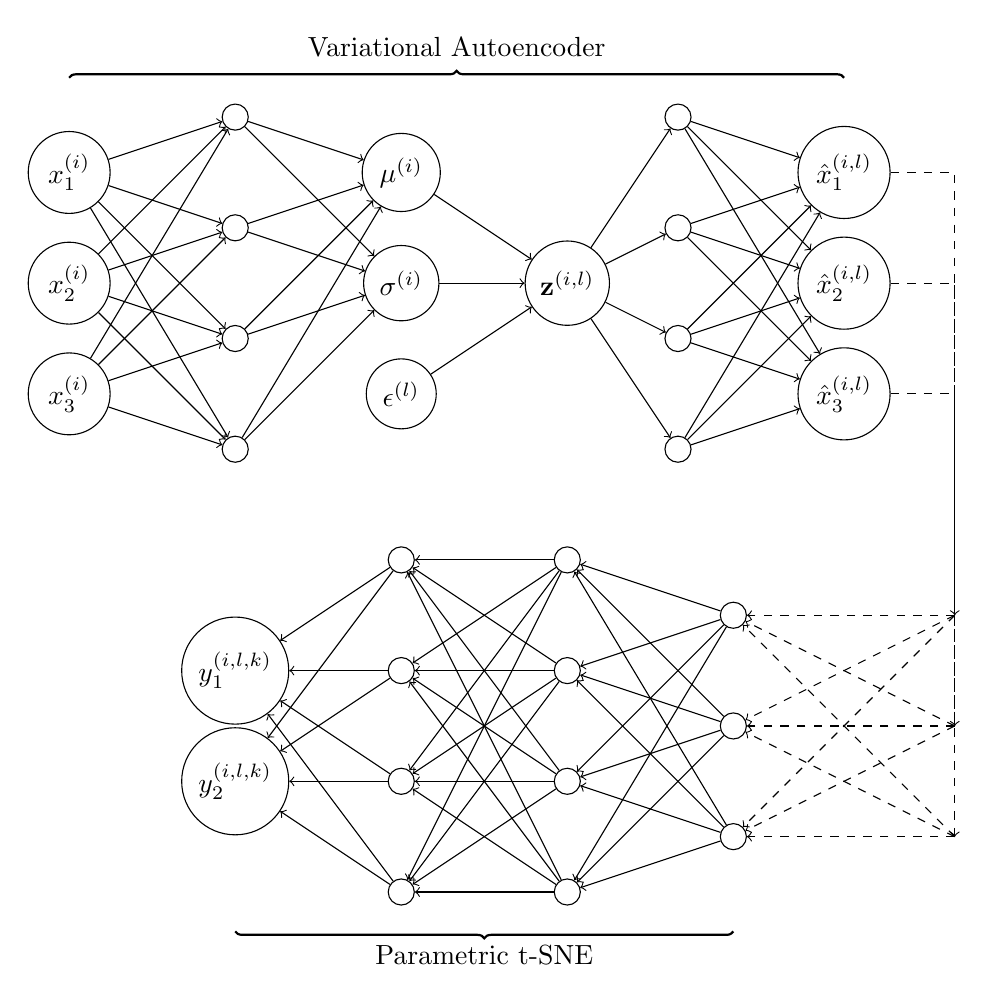
\begin{tikzpicture}[x=1em,y=1em]

  % VAE
  % Input layer
  \foreach \i in {1,...,3}{
    \node[draw, circle] (N-1-\i) at (0, 10 + 4 - 4 * \i) {$x^{(i)}_{\i}$};
  }
  % Encoder hidden layer
  \foreach \i in {1,...,4}{
    \node[draw, circle] (N-2-\i) at (6, 12 + 4 - 4 * \i) {};
    \foreach \j in {1,...,3}{
      \draw [->] (N-1-\j) -- (N-2-\i);
    }
  }
  % Latent code
  \node[draw, circle] (mu) at (12, 10) {$\mathbf{\mu}^{(i)}$};
  \node[draw, circle] (sigma) at (12, 6) {$\mathbf{\sigma}^{(i)}$};
  \node[draw, circle] (eps) at (12, 2) {$\mathbf{\epsilon}^{(l)}$};
  \node[draw, circle] (z) at (18, 6) {$\mathbf{z}^{(i, l)}$};
  \foreach \x in {mu,sigma,eps}{
    \draw [->] (\x) -- (z);
  }
  \foreach \x in {mu,sigma}{
    \foreach \j in {1,...,4}{
      \draw [->] (N-2-\j) -- (\x);
    }
  }
  % Decoder hidden layer
  \foreach \i in {1,...,4}{
    \node[draw, circle] (N-4-\i) at (22, 12 + 4 - 4 * \i) {};
    \draw [->] (z) -- (N-4-\i);
  }
  % Output layer
  \foreach \i in {1,...,3}{
    \node[draw, circle] (N-5-\i) at (28, 10 + 4 - 4 * \i) {$\hat{x}^{(i, l)}_{\i}$};
    \foreach \j in {1,...,4}{
      \draw [->] (N-4-\j) -- (N-5-\i);
    }
  }

  % PTSPE
  % Input layer
  \foreach \i in {1,...,3}{
    \node[draw, circle] (P-1-\i) at (24 + 0, -16 + 10 + 4 - 4 * \i) {};
  }
  % Hidden layer 1
  \foreach \i in {1,...,4}{
    \node[draw, circle] (P-2-\i) at (24 - 6, -16 + 12 + 4 - 4 * \i) {};
    \foreach \j in {1,...,3}{
      \draw [->] (P-1-\j) -- (P-2-\i);
    }
  }
  % Hidden layer 2
  \foreach \i in {1,...,4}{
    \node[draw, circle] (P-3-\i) at (24 - 12, -16 + 12 + 4 - 4 * \i) {};
    \foreach \j in {1,...,4}{
      \draw [->] (P-2-\j) -- (P-3-\i);
    }
  }
  % Output layer
  \foreach \i in {1,...,2}{
    \node[draw, circle] (P-4-\i) at (24 - 18, -16 + 8 + 4 - 4 * \i) {$y_{\i}^{(i,l,k)}$};
    \foreach \j in {1,...,4}{
      \draw [->] (P-3-\j) -- (P-4-\i);
    }
  }

  \foreach \i in {1,...,3}{
    \coordinate (C-\i) at (32, -16 + 10 + 4 - 4 * \i);
    \draw [dashed,->] (N-5-\i) -| (C-\i);
    \foreach \j in {1,...,3}{
      \draw [dashed,->] (C-\i) -- (P-1-\j);
    }
  }

  \draw [thick, decoration={brace, raise=0.5cm}, decorate] (0,12) -- (28,12) node[pos=0.5,anchor=north,yshift=1.15cm] {Variational Autoencoder};
  
  \draw [thick, decoration={brace, mirror, raise=0.5cm}, decorate] (6,-16) -- (24,-16) node[pos=0.5,anchor=north,yshift=-0.55cm] {Parametric t-SNE};

\end{tikzpicture}
\unskip}
  \caption{Illustration of the general structure of a VPTSNE network.}
  \label{fig:vptsne}
\end{figure}

\begin{algorithm}[H]
  \caption{Training of the neural networks.}
  \label{alg:learning}
  \begin{algorithmic}[1]
    \Require Data set $\mathbf{D}$ of size $N$, VAE training batch size $M_{\mathsf{VAE}}$, VAE samples $L$, PTSNE training batch size $M_{\mathsf{PTSNE}}$
    \Ensure Neural network parameters $\btheta, \bphi, \bW$
    \State $\btheta, \bphi, \bW \gets \text{Initialize neural network parameters}$
    \While{VAE not converged}
      \State $\mathbf{X} \gets \text{ Random minibatch of size } M_{\mathsf{VAE}} \text{ from } \mathbf{D}$
      \ForAll{$\bxi \in \mathbf{X}$}
        \For{$l \gets 1$ to $L$}
          \State $\eil \gets \text{ Draw sample from noise distribution } p(\beps)$
          \State $\bz^{(i,l)} \gets g_{\bphi}(\bxi, \eil)$ \Comment{Draw from $\qphi(\bz \vert \bxi)$}
          \State $\hat{\bx}^{(i,l)} \gets f_{\btheta}(\bzil)$ \Comment{Obtain parameters of $\ptheta(\bx \vert \bzil)$ by decoding $\bzil$}
        \EndFor
        \State $\mathcal{L}(\btheta, \bphi; \bxi) \gets \text{ Compute estimate with either equation \ref{eq:vae_loss} or \ref{eq:vae_loss_2} }$
      \EndFor
      \State $\btheta, \bphi \gets \text{ Updata parameters by ascending gradient } \nabla_{\btheta, \bphi} \frac{N}{M_{\mathsf{VAE}}} \sum_{i=1}^{M_{\mathsf{VAE}}} \mathcal{L}(\btheta, \bphi; \bxi)$
    \EndWhile
    \While{PTSNE not converged}
      \State $\mathbf{X} \gets \text{ Random minibatch of size } M_{\mathsf{PTSNE}} \text{ from } \mathbf{D}$
      \ForAll{$\bxi \in \mathbf{X}$}
        \State $\eil \gets \text{ Draw sample from noise distribution } p(\beps)$
        \State $\bz^{(i,l)} \gets g_{\bphi}(\bxi, \eil)$ \Comment{Draw from $\qphi(\bz \vert \bxi)$}
        \State $\widetilde{\bx}^{(i)} \gets \text{ Draw sample from } \ptheta(\bx \vert \bzil)$ \Comment{Obtain reconstruction from VAE}
        \State $\mathbf{y}^{(i)} \gets f_{\bW}(\widetilde{\bx}^{(i)})$
      \EndFor
      \State $\bW \gets \text{ Update parameters by descending gradient } \nabla_{\bW} C_{\text{t-SNE}} \text{ using } \widetilde{\bx}^{(i)} \text{ and } \mathbf{y}^{(i)}$
    \EndWhile
  \end{algorithmic}
\end{algorithm}

\note{As we can draw infinite samples from the continuous distribution $p_{\bphi}(\bz \vert \bxi)$ with $g_{\bphi}(\bxi, \eil)$ ...}

After training, a deterministic projection for all subsequent points can be obtained with Algorithm~\ref{alg:projection}. For encoder and decoder network pairs that both directly parameterize the mean of a distribution, computing the expectation can be done exactly with zero overhead.

\begin{algorithm}[H]
  \caption{Deterministic projection.}
  \label{alg:projection}
  \begin{algorithmic}[1]
    \Require Point $\bxi$, neural network parameters $\btheta, \bphi, \bW$
    \Ensure Projected point $\mathbf{y}^{(i)}$
    \State $\widetilde{\bz}^{(i)} \gets \mathbb{E}[\qphi(\bz \vert \bxi)]$
    \State $\widetilde{\bx}^{(i)} \gets \mathbb{E}[\ptheta(\bx \vert \widetilde{\bz}^{(i)})]$
    \State $\mathbf{y}^{(i)} \gets f_{\bW}(\widetilde{\bx}^{(i)})$
  \end{algorithmic}
\end{algorithm}

\section{Obtaining Reconstructions from Hidden Layers}
\label{section:sampling_from_hidden_layers}

Instead of training the embedding network on the final output of the VAE it is possible to instead use the outputs of a chosen hidden layer. If the chosen hidden layer has dimensions considerably smaller than that of the original, the benefits of this approach are twofold:

\begin{itemize}
\item We are performing a step of nonlinear dimensionality reduction that is not dependent on distance metrics, i.e. a preprocessing step that is less susceptible to the curse of dimensionality.
\item Given that the number of dimensions can be chosen to be considerably lower than in the original input space, computing the t-SNE loss also becomes proportionally cheaper.
\end{itemize}

When considering precomputed $P_{ij}$ matrices for each batch the gain in computational advantage does however diminish significantly, although the following caveats apply to the precomputation. Storing the precomputed matrices will require considerable space for large batch sizes and data sets. A way to circumvent the need for large storage space is to employ a k-NN approximation when computing $P_{ij}$, i.e. only considering a small number of neighbors when computing the conditional probabilities for each pair of points, which will result in a sparse matrix. This however increases the error in the computed gradient and relies on an efficient k-NN algorithm in practice, which require the use of approximation algorithms when the data's dimensionality is high, as the use of space partitioning data structures for exact k-NN becomes computationally intractable. Additionally, fixing the batches in advance hinders the performance of SGD as the gradient estimates become biased. Moreover, relying on precomputed $P_{ij}$ matrices for fixed batches prevents the use of infinite sample generation from the VAE.

\section{Inference with the Generative Model}
\label{section:inference_with_the_generative_model}

From the underlying generative model we can estimate the marginal likelihood $p(\bx)$ for each data point $\bx$. An estimation can be retrieved by importance sampling \cite{stochastic_backpropagation}:

$$p(\bx) \simeq \frac{1}{N} \sum_{i=1}^{N} \frac{p(\bx \vert \bz^{(i)}) p(\bz^{(i)})}{q_{\theta}(\bz^{(i)} \vert \bx)},$$

where $\bz^{(i)} \sim q_{\theta}(\bz \vert \bx)$. Alternatively, one could directly use the ELBO to estimate $p(\bx)$; however, this gives generally worse estimates \cite{ais_vae}. For more accurate estimates than importance sampling, the usage of annealed importance sampling \cite{ais} has been suggested for VAEs in \cite{ais_vae}.

Using the obtained marginals as feedback we can inform the user of potentially anomalous points in the data set. This feedback can then further be used in downstream analysis. From a data visualization perspective, points that do not fit the model well correspond to points that are likely to be mapped poorly, thus removing such outliers from the final mapping serves to highlight the natural clusters in the data more clearly.

\section{Robustness to Sparse and Noisy Data}
\label{section:robustness}

\note{The unknown intrinsic dimensionality of the data manifold is reduced to at most the dimensionality of the latent code. Data less sparsely distributed on this manifold.}
\note{The stochastic model allows sampling infinitely many points on the learned manifold.}

As real-world data is generally not perfectly clean, an important property for any machine learning method is its capability to handle data containing artifacts. Considering VAEs are inherently robust to corrupted data due to the regularization provided by the stochastic latent code (\textcolor{red}{[connection with VAE and Robust PCA \cite{rpca_1, rpca_2} shown in \citep{hidden_talents_of_the_vae}]}) it is reasonable to hypothesize that a training procedure for a low dimensional mapping taking advantage of this property would perform better on corrupted data.

\section{Implementation}
\label{section:implementation}

An accompanying implementation of the method has been made available at \url{https://github.com/ahie/vptsne}. The implementation is built on top of TensorFlow \cite{tensorflow} and takes advantage of the TensorFlow Distributions \cite{tensorflow_distributions} library. To take full advantage of the dataflow architecture of TensorFlow and the paralellism provided by GPUs, both the t-SNE loss and its gradient computation were implemented as custom CUDA \cite{cuda} kernel operations.

The implementation has been made as extensible as possible by allowing the full specification of the neural network structures parameterizing the VAE distributions and the PTSNE network. Helpers for easily specifying common network structures are included in the implementation. The use of normalizing flows in the VAE model has also been made possible. Additionally, the fast approximate nearest neighbor algorithm NN-descent \cite{nn_descent} has been included in the t-SNE CUDA routines as an optional performance enhancement for computing the input space distribution $P_{ij}$ when training with large batch sizes.

\chapter{Experiments}
\label{ch:experiments}

Several experiments are carried out to validate the efficacy of the method outlined in this thesis. The learning of a parametric embedding using our method is compared to plain PTSNE. Other methods of dimensionality reduction are compared against our method in terms of both embedding quality and scalability. Additionally, robustness properties of the method are demonstrated empirically as well as training the embedding on hidden layer outputs is experimented with. Lastly, two applications of the method to single cell data analysis are presented in section \ref{section:applications}, including a demonstration of the use of the VAE for inference.

Before going into the results and applications of the method this chapter begins by first presenting the different data sets that will be used throughout the experiments after which the different quantitative metrics for evaluating the experimental results are covered and the general experimental setup, in regards to the used network structures, parameters and chosen optimization methods are discussed.

\section{Data Sets}

The five different data sets described below were used to conduct the experiments of this section.

\subsection{MNIST}

The MNIST data set \cite{mnist} contains labeled images of handwritten digits. Each image contains a single digit in gray-scale with a resolution of 28x28 pixels. The data set is split into $60000$ training images and $10000$ test images. All networks were trained solely on the training data set, while the remaining test examples were reserved for assessing the capability of the network to generalize to out-of-sample extensions. In the unsupervised setting considered here, the provided labels were only used for visualizing the embeddings and evaluating the embedding quality of out-of-sample extensions via a 1-NN classifier.

MNIST is a standard data set that frequently appears in machine learning literature and is regularly included in unsupervised learning experiments. As a relatively simple labeled real-world data set it functions as a good baseline for studying the output of our method.

\subsection{Fashion-MNIST}

The Fashion-MNIST data set \cite{fashion_mnist} was designed as a drop-in replacement for the MNIST data set and thus contains the same number of grayscale training and test images of equal dimensions. The images themselves consist of 10 different classes of fashion items, such as T-shirts, trousers, sneakers, and handbags. The motivation for considering this data set in addition to MNIST is the fact that it has been shown to be harder to learn even with supervised computer vision methods.

\subsection{Mass Cytometry}

Cytometry is the measurement of biological characteristics of cells. In mass cytometry, time-of-flight mass spectrometry is used to measure the counts of cellular proteins present within a single cell by tagging proteins with their corresponding antibodies that have been conjugated with specific heavy metals.

As a comparatively new methodological development, mass cytometry enables simultaneous measurement of a considerably greater number of features compared to fluorescence-based flow cytometry. A greater number of features, however, poses new challenges in analyzing the measurement results. To aid the analysis of this high dimensional data it is common to visualize the data as a 2-D or 3-D scatter plot using t-SNE, due to its capability to separate biologically relevant subpopulations of cells in the produced embedding \cite{visne}. However, as a high-throughput method, mass cytometry data sets under analysis can grow to be millions of data points in size, prompting the use of more scalable algorithms. For a more thorough review of mass cytometry and associated analytical challenges, the reader is referred to \cite{mass_cytometry}.

In our experiments, we consider two different mass cytometry data sets. As the first data set, henceforth referred to as Cytometry A, we use the publicly available data of \cite{phenograph}, which has been used to demonstrate the effectiveness of the Phenograph clustering algorithm on mass cytometry data. The data set consists of $81000$ data points of $13$ dimensions corresponding to the normalized counts of cell surface proteins belonging to distinct clusters of differentiation. As a benchmark data set for the Phenograph clustering algorithm, we additionally include the labels produced by Phenograph in our analysis.

The second mass cytometry data set (Cytometry B) contains data gathered from ovarian cancer patients at different phases of treatment. The number of points in the entire data set is $1.4$ million, each of which has $23$ dimensions.

\subsection{Single-Cell RNA Sequencing}

Single-cell RNA sequencing (scRNA-seq) enables the measurement of the transcriptional state of single cells. By mapping sequenced RNA fragments present in a given cell to RNA sequences of predetermined genes the expression profile of tens of thousands of genes can be measured simultaneously with current high-throughput sequencing methods. As the number of genes for which the strength of expression can be quantified is far greater than the number of proteins that can be measured with mass cytometry the computational and analytical challenges are further exacerbated \cite{high_dimensional_data_spaces_gene_and_protein, computational_challenges_single_cell_transcriptomics}.

We explore how our method applied to scRNA-seq data reveals biologically meaningful insights by applying it to the melanoma patient data set studied in \cite{tirosh}. The data set consists of tumor samples from $19$ different patients, altogether containing $4097$ cells for which the expression of $22462$ genes is measured. The data set additionally includes labels for each cell denoting their cell type and tumor of origin.

\section{Evaluation Metrics}

To quantitatively evaluate the quality of embeddings two different measures are used in this work. By quality of the embeddings we are interested in how well the local structure of the data is preserved. The choice of the two metrics used in this work follows those used in the original work on parametric t-SNE \cite{parametric_tsne}. A short description for each is given below.

\subsection{k-Nearest Neighbor Classifier}

Given a labeled data set a k-nearest neighbor (k-NN) classifier can be used to roughly assess how well different classes are separated in the output space of an embedding. A k-NN classifier works simply by returning the majority label of a given point's k-nearest neighbors in the training data set. For example in the 1-NN classifier case, the decision boundary can be geometrically visualized as a Voronoi diagram as in Figure~\ref{fig:voronoi}.

Throughout the experiments, the performance of nearest neighbor classifiers in the output space of embeddings will be evaluated. More precisely, the accuracy of a 1-nearest neighbor classifier with the Euclidean metric for determining neighbor distance is used.

For parametric methods, the classifier can be trained on the embedding of training data points and separately tested on the training set. This enables evaluating the ability of the embedding function to generalize to unseen data. On the other hand, for non-parametric methods, the final embedded data points need to be split into train and test sets for the 1-NN classifier.

\begin{figure}[!htb]
  \centering
  \resizebox{0.5\textwidth}{!}{\def\n{10}
\def\maxxy{4}
\def\biglen{20cm}
\tikzset{
  half plane/.style={ to path={
       ($(\tikztostart)!.5!(\tikztotarget)!#1!(\tikztotarget)!\biglen!90:(\tikztotarget)$)
    -- ($(\tikztostart)!.5!(\tikztotarget)!#1!(\tikztotarget)!\biglen!-90:(\tikztotarget)$)
    -- ([turn]0,2*\biglen) -- ([turn]0,2*\biglen) -- cycle}},
  half plane/.default={1pt}
}

\begin{tikzpicture}[x=1em,y=1em]

  % generate random points
  \pgfmathsetseed{2018}
  \def\pts{}
  \xintFor* #1 in {\xintSeq {1}{\n}} \do{
    \pgfmathsetmacro{\ptx}{.9*\maxxy*rand} % random x in [-.9\maxxy,.9\maxxy]
    \pgfmathsetmacro{\pty}{.9*\maxxy*rand} % random y in [-.9\maxxy,.9\maxxy]
    \edef\pts{\pts, (\ptx,\pty)} % stock the random point
  }
  
  % draw the points and their cells
  \xintForpair #1#2 in \pts \do{
    \edef\pta{#1,#2}
    \begin{scope}
      \xintForpair \#3#4 in \pts \do{
        \edef\ptb{#3,#4}
        \ifx\pta\ptb\relax % check if (#1,#2) == (#3,#4) ?
          \tikzstyle{myclip}=[];
        \else
          \tikzstyle{myclip}=[clip];
        \fi;
        \path[myclip] (#3,#4) to[half plane] (#1,#2);
      }
      \clip (-\maxxy,-\maxxy) rectangle (\maxxy,\maxxy); % last clip
      \pgfmathsetmacro{\randhue}{rnd}
      \definecolor{randcolor}{hsb}{\randhue,.5,1}
      \fill[randcolor] (#1,#2) circle (4*\biglen); % fill the cell with random color
      \fill[draw=black,very thick] (#1,#2) circle (1.5pt); % and draw the point
    \end{scope}
  }
  
  \pgfresetboundingbox
  \draw[opacity=0] (-\maxxy,-\maxxy) rectangle (\maxxy,\maxxy);
\end{tikzpicture}
\unskip}
  \caption{Voronoi diagram illustrating the decision boundaries of 10 different classes of a 1-NN classifier. Black dots represent the training data points, and the different colors correspond to the label of the data point for that region. Any point to be classified would receive the label corresponding to the location in the tesselation it lies on. The distance metric used in this example is the Euclidean distance.}
  \label{fig:voronoi}
\end{figure}

\subsection{Trustworthiness}

Trustworthiness, introduced by Venna et al. \cite{trustworthiness}, is a measure of the degree to which local structure is preserved in the output space relative to the input space after dimensionality reduction is performed. Trustworthiness has been used to compare multiple dimensionality reduction methods for the purposes of visualization of high dimensional data sets such as gene expression data \cite{trustworthiness_gene_expression} and gene interaction graphs \cite{trustworthiness_gene_interaction}.

Computation of trustworthiness is done by comparing how the rank order for each point's $k$ nearest neighbors in the output space match that of the input space. Formally, for a chosen number $k$ of neighbors it is given by the following 

$$T(k) = 1 - \frac{2}{nk (2n - 3k - 1)} \sum^{n}_{i=1} \sum_{j \in \mathcal{N}_{i}^{k}} (r(i, j) - k),$$

where $n$ is the total number of data points under consideration, $\mathcal{N}_{i}^{k}$ is the set of $k$ nearest neighbors in the output space of data point $i$, and $r(i, j)$ is a function giving the rank of node $j$ in the nearest neighbor ordering of node $i$. The possible values for trustworthiness range from 0 to 1, indicating complete loss of local structure and perfect preservation of local structure, respectively.

\section{Network Structure and Parameters}
\label{section:network_structure_and_parameters}

To parameterize the embedding $f(\mathbf{\hat{x}})$ a feedforward neural network with layers of hidden units with dimensions $d - 500 - 500 - 2000 - 2$ were used, where $d$ is the input dimensionality and rectifier linear unit (ReLU) activations are applied to the hidden unit outputs to induce nonlinearity to the network. The hidden unit dimensions were chosen to match those of the final combined network used in \cite{parametric_tsne}, although we have substituted the sigmoid activations with ReLU activations. Furthermore, we do not perform stacked restricted Boltzmann machine pretraining on the hidden layer weights as in \cite{parametric_tsne}. However we do benchmark the performance of our network against the original parametric t-SNE implementation. Since we are not considering RBM pretraining and are instead relying on the property of ReLUs reducing the vanishing gradient problem \cite{relu} and better initialization \cite{xavier_initializer}. Running the original implementation shows little benefit in performing this costly initialization. We could instead reuse the trained encoder weights of the VAE as a starting point for the optimization of our embedding network.

For optimization of the neural network \cite{parametric_tsne} use nonlinear conjugate gradient descent, whereas Adam \citep{adam} is used as the optimizer in the results presented here. Updates with Adam are considerably faster to compute than with conjugate gradient descent. Throughout all experiments standard parameters for Adam were chosen, i.e. a learning rate of $0.001$ and the exponential decay rates of the 1st and 2nd moments were set to $0.9$ and $0.999$ respectively. The more recent optimizer AMSGrad \cite{on_the_convergence_of_adam} was considered, but due to little evidence of its benefit over Adam when used in non-synthetic optimization problems its use was left for future work.

We applied batch normalization \cite{batch_normalization} to the hidden layers of the VAE networks, while omitting batch normalization from the embedding network. This is to validate the training procedure on as simple an embedding network as possible. We note that applying batch normalization to the embedding network improves the results marginally.

To further emphasize the universality of our approach we restrict ourselves to use a simple VAE structure, without complicating the model architecture with more recently proposed advances, such as normalizing flows.\footnote{In preliminary results VAE models that achieve a lower ELBO do in fact contribute to improved embeddings.} Throughout all experiments, unless otherwise specified, the VAE architecture was fixed to $d - 256 - 128 - 32 - \mu, \log \sigma^2 - 32 - 128 - 256 - d$, where $\mu$ and $\sigma$ parameterize a normal distribution acting as the posterior $q_{\phi}(\bz \vert \bx^{(i)})$ and the final layer output was used to parameterize a Bernoulli distribution for MNIST as well as Fashion-MNIST, and a Gaussian distribution with a fixed standard deviation of 0.1 for cytometry data. In all experiments, each VAE was trained with a batch size of 1000 for 10000 iterations and had a latent dimensionality of $3$, unless otherwise specified.

For MNIST and Fashion-MNIST perplexities were set to 30, which is in line with the value used by \cite{parametric_tsne}, whereas for the mass cytometry and scRNA-seq data sets a perplexity of 10 was chosen. It should be noted that a more correct way to choose perplexity would take into account the batch size, as perplexity controls the number of neighbors each point is considered to have. For example training VPTSNE on MNIST with batch size 200 and perplexity 10 gives better results than with perplexity 30. However, with PTSNE the results are actually worse as the training fails to converge even with small learning rates. An example embedding of MNIST with low perplexity and small batch size has been included in Appendix~\ref{appendix:low_perp_small_bs}, which achieves better trustworthiness (0.935) and 1-NN (0.812) than the 600 batch size, 30 perplexity runs. Why PTSNE fails to converge and VPTSNE does not is an important question to explore in future work, as this demonstrates a clear advantage of the method being proposed.

Degrees of freedom of the t-Distribution for the PTSNE objective was set to 1 throughout all experiments, as all embeddings performed were two-dimensional.

\section{Results}
\label{section:results}

\subsection{Learning}
\label{subsection:learning}

In this section we compare the effect of training on VAE reconstructions to training on the original MNIST data set. To quantitatively evaluate the quality of the embeddings produced we employed the trustworthiness metric \cite{trustworthiness} on the MNIST test set. Additionally, we compared the 1-NN classification errors by fitting the classifiers on the produced embeddings of the training set and finding the mean accuracies of the classifiers on the test set.

In figure \ref{fig:mnist_knn_trustworthiness} we have plotted the 1-NN scores and trustworthiness of the embeddings obtained after each iteration of training for two different batch sizes. The runs for each batch size were repeated 20 times, plotting the means and 95\% confidence intervals of the means. Training with VAE reconstructions shows a clear improvement both qualitatively and quantitatively over training on the original data when small training batches are used to approximate the t-SNE loss gradient. Higher trustworthiness, as well as 1-NN scores are obtained consistently and convergence is reached in fewer iterations. Moreover, the results are in favor of training on reconstructions by exhibiting more stable results during training.

Qualitatively the embeddings trained on the original data remain noisier than the embeddings trained on the reconstructed data points. This can be seen in figure \ref{fig:mnist_comparison}, where the separation of true clusters in the embedding is less evident, with several classes overlapping and a large number of outlier points for each class. We further compare the qualitative differences of the embeddings produced with the Fashion-MNIST dataset. In figure \ref{fig:fashion_mnist_comparison} similar deficiencies in the embedding can be noted as in the embedding comparisons for the MNIST data set. In particular, the visible clusters of classes are less distinct, as well as the global layout of the classes is considerably worse, e.g. the cluster of footwear related images has been pulled closer to the cluster of upper body garments and the images of bags have been split into two seemingly unrelated clusters.

\begin{figure}[!htb]
  \centering
  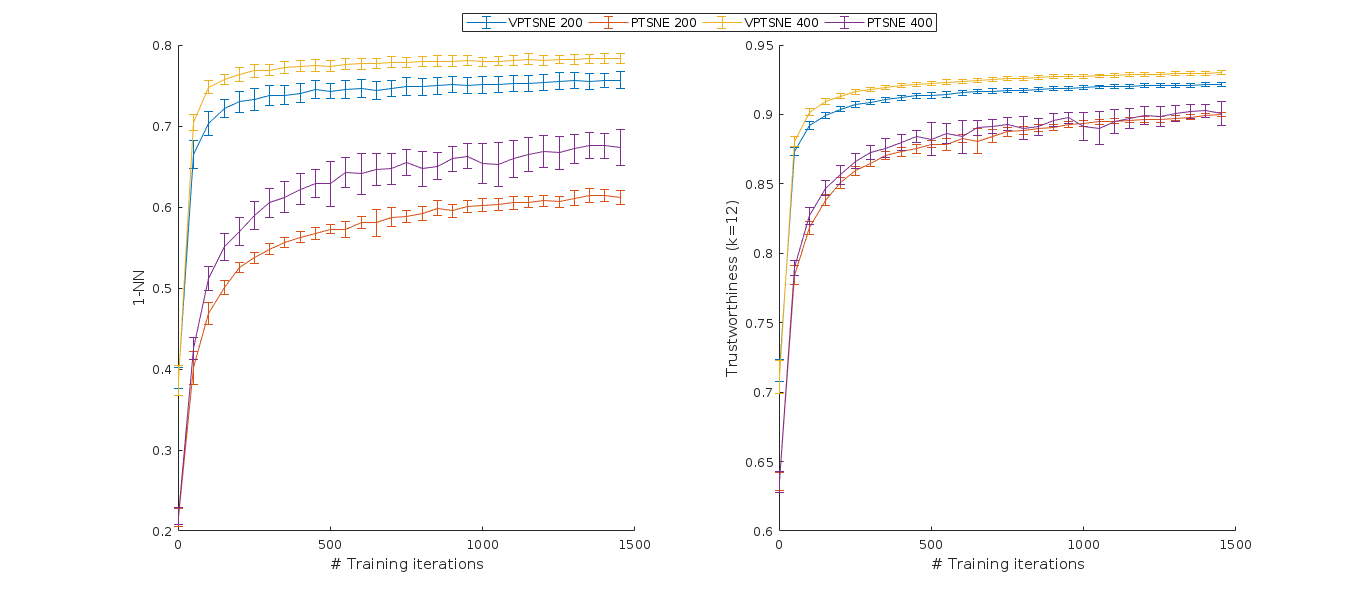
\includegraphics[width=\textwidth]{images/learning_curves.png}
  \caption{Plots of 1-NN and trustworthiness scores obtained after a given number of iterations for different batch sizes. The means and 95\% confidence intervals of the means have been plotted from 20 repeated runs for each parameter setting.}
  \label{fig:mnist_knn_trustworthiness}
\end{figure}

\begin{figure}[!htb]
  \centering
  \begin{tabular}{cc}
    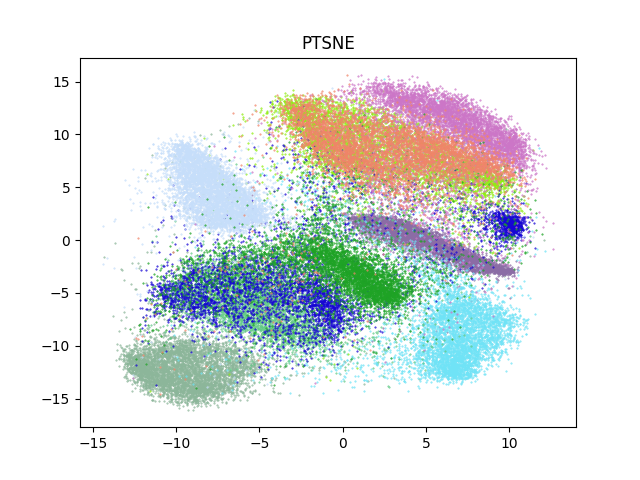
\includegraphics[width=0.45\textwidth]{images/mnist_ptsne_embedding.png} &
    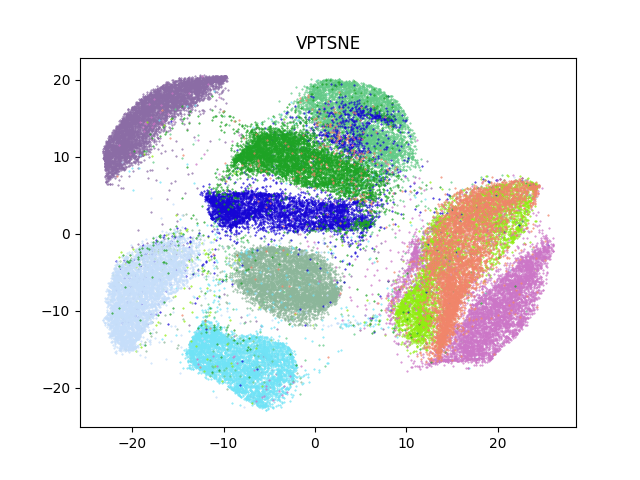
\includegraphics[width=0.45\textwidth]{images/mnist_vptsne_embedding.png} \\
    \multicolumn{2}{c}{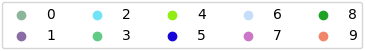
\includegraphics[width=0.45\textwidth]{images/mnist_legend.png}}
  \end{tabular}
  \caption{Embeddings of the MNIST data set trained with batch size 400.}
  \label{fig:mnist_comparison}
\end{figure}

\begin{figure}[!htb]
  \centering
  \begin{tabular}{cc}
    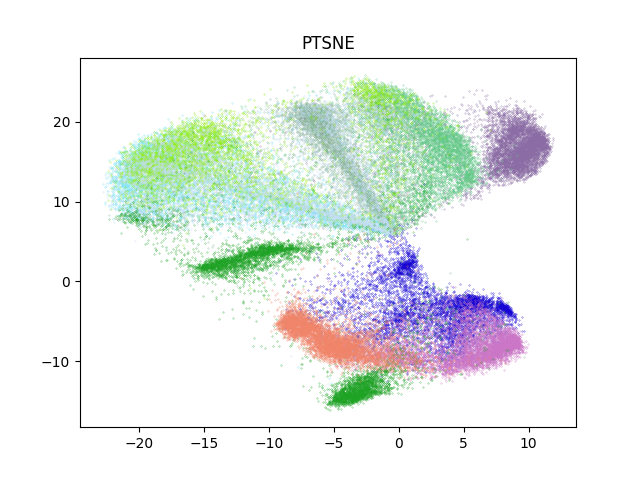
\includegraphics[width=0.45\textwidth]{images/fashion_mnist_ptsne_embedding.png} &
    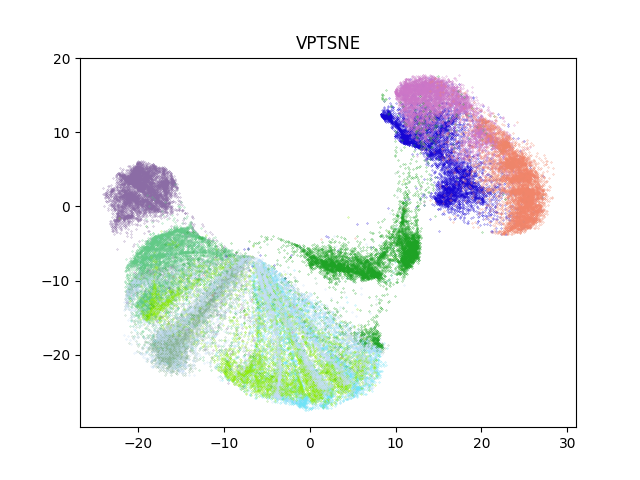
\includegraphics[width=0.45\textwidth]{images/fashion_mnist_vptsne_embedding.png} \\
    \multicolumn{2}{c}{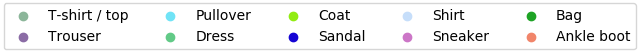
\includegraphics[width=0.45\textwidth]{images/fashion_mnist_legend.png}}
  \end{tabular}
  \caption{Embeddings of the Fashion-MNIST data set trained with batch size 400.}
  \label{fig:fashion_mnist_comparison}
\end{figure}

\subsection{Comparisons}
\label{section:comparisons}

We now compare the proposed method to other parametric dimensionality reduction methods, namely PCA and VAE. In addition we also consider two non-parametric dimensionality reduction methods, t-SNE and the recently proposed method UMAP \cite{umap}, which had been demonstrated to be able to produce embeddings comparable to t-SNE while being more efficient to optimize in practice.

For the comparisons we will be using the Cytometry A data set. As evaluation criteria, similarly to the previous section, both trustworthiness and 1-NN classification accuracy are used. In addition to comparing the quality of the embeddings, the runtime performance of the different methods are studied. Our goal is to demonstrate that our method produces competitive embeddings as well as has superior scalability.

\subsubsection{Embedding Quality}
\label{subsubsection:embedding_quality}

The quantitative results for all methods under comparison are available in table \ref{table:comparison} and the corresponding scatter plots of the 2-D embeddings are presented in figure \ref{fig:comparison_figure}. Although VAE produces quantitatively better results for the chosen metrics, the spatial layout of clusters in the resulting embedding have less distinct separation and the global structure of the embedding is constrained by the chosen prior $p(\bz)$. From a data visualization standpoint these factors make the latent space embeddings qualitatively worse than what the corresponding quantitative metrics would suggest. Unsurprisingly, PCA performs the worst on both quantitative and qualitative results. Our method however is able to reach results on par with those of the chosen non-parametric methods.

It can also be observed that t-SNE, with the given perplexity, preserves global structure much more poorly. This can be observed by comparing with the PCA plot, which has three clearly distinct, spatially separated clusters of clusters that are not present in the t-SNE plot.

The effect of choosing a suitable perplexity w.r.t. batch size mentioned in Section~\ref{section:network_structure_and_parameters} was noted in these experiments. With large perplexity the clusters in the t-SNE embedding begin to separate more distinctly like with VPTSNE and UMAP, but here the same perplexity is used for both VPTSNE and t-SNE optimization. As perplexity is increased t-SNE optimization becomes considerably slower, for example going from perplexity 10 to 100 increased the total computation time twofold.

\subsubsection{Scalability}
\label{subsubsection:scalability}

A major practical challenge with nonlinear dimensionality reduction methods are their scalability to large data sets. Typically, to capture the spatial structure of data a distance metric is employed to compute the pairwise distances for the entire data set, after which a projection of the points to a lower dimensional space, equipped with a corresponding metric, is sought that retains the computed distances as accurately as possible. As the number of data points increases, the inherent quadratic complexity of methods relying on such pairwise distance computations quickly renders such methods intractable.

In practice, various approximations and data structures are employed to speed up dimensionality reduction methods. With t-SNE a widely used performance enhancement, independently investigated by Yang et al. \cite{accelerated_tsne_1} and van der Maaten \cite{accelerated_tsne_2}, is to use the Barnes-Hut algorithm \cite{barnes_hut} to approximate the $Q_{ij}$ matrix by averaging the influence of distant points belonging to the same node in the underlying space partitioning data structure. This approximation nevertheless fails to provide significant speedup in the general case depending on the chosen tradeoff between accuracy and speed, as well as the distribution of the points being optimized at each step. Furthermore, its use is limited to obtaining 2 or 3 dimensional embeddings due to its use of the quadtree and octree data structures for each respective dimensionality. On the other hand, optimization of the parametric embedding can be performed with stochastic gradient descent. As we have shown, even with small batch sizes we are able to produce embeddings of competitive quality. The Barnes-Hut approximation can also be used to further speed up the computation of the loss and its gradient, but for small batch sizes the computational overhead of constructing the required data structure can outweigh the cost of directly computing all pairwise influences within the batch. Direct computation has the additional benefit that it is not limited to output dimensionalities for which a space partitioning data structure can be efficiently built.

As previously mentioned, one of the strengths of UMAP compared to t-SNE is the efficiency of its optimization. The key to its efficient optimization is that its gradient can be approximated stochastically via probabilistic edge sampling following the procedure introduced in \cite{largevis}. As both VPTSNE and UMAP take advantage of stochastic gradient descent, the scalability of their optimization is equal up to an implementation dependent constant factor. VPTSNE however maintains the advantage over UMAP that natural out-of-sample extension is made possible through the learned embedding function.

\begin{table}[]
\centering
\caption{Comparison between different dimensionality reduction methods.}
\label{table:comparison}
\begin{tabular}{cccc}
Algorithm   & Trustworthiness ($k=12$)   & 1-NN     & time (ms) \\ \hline \hline
VPTSNE      & $0.9753$                   & $0.9250$ & $60766$   \\ \hline
PTSNE       & $0.9628$                   & $0.8890$ & $8729$    \\ \hline
UMAP        & $0.9688$                   & $0.9297$ & $74716$   \\ \hline
VAE         & $0.9762$                   & $0.9247$ & $52037$   \\ \hline
t-SNE       & $0.9879$                   & $0.9536$ & $1192812$ \\ \hline
PCA         & $0.8557$                   & $0.4886$ & $96$      \\ \hline
\end{tabular}
\end{table}

\begin{figure}[!htb]
  \centering
  \begin{tabular}{cccc}
    VPTSNE &
    \raisebox{-.5\height}{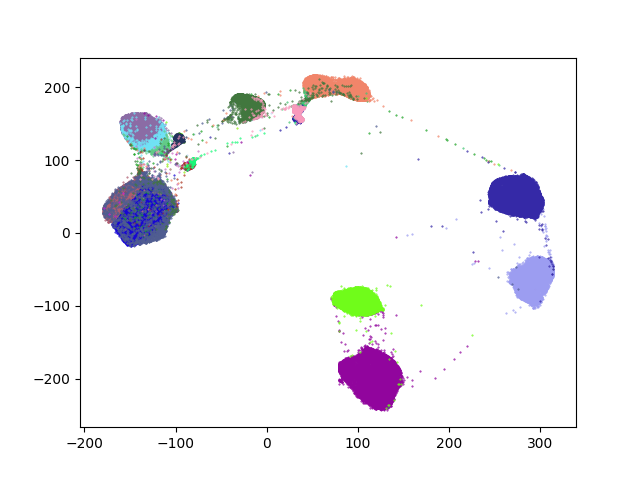
\includegraphics[width=0.25\textwidth]{images/vptsne_levine.png}} &
    \raisebox{-.5\height}{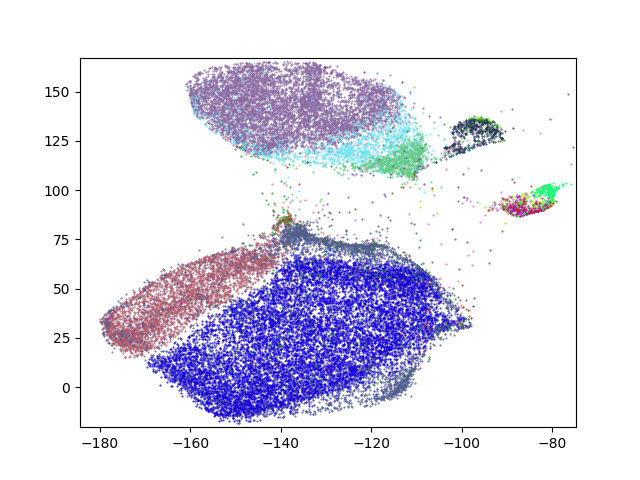
\includegraphics[width=0.25\textwidth]{images/vptsne_levine_zoomed.png}} &
    \raisebox{-.5\height}{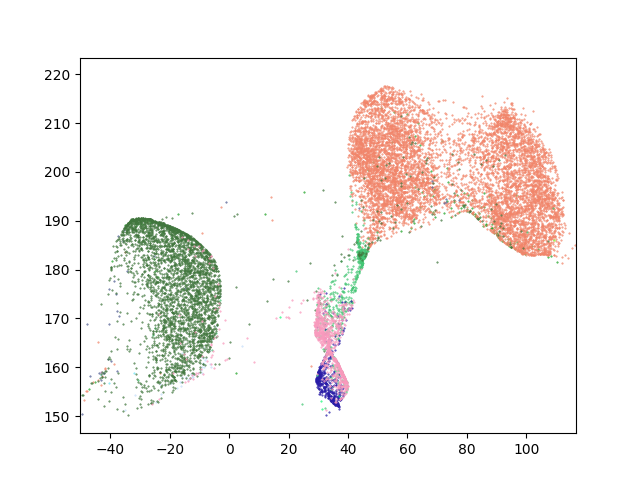
\includegraphics[width=0.25\textwidth]{images/vptsne_levine_zoomed_2.png}} \\
    PTSNE &
    \raisebox{-.5\height}{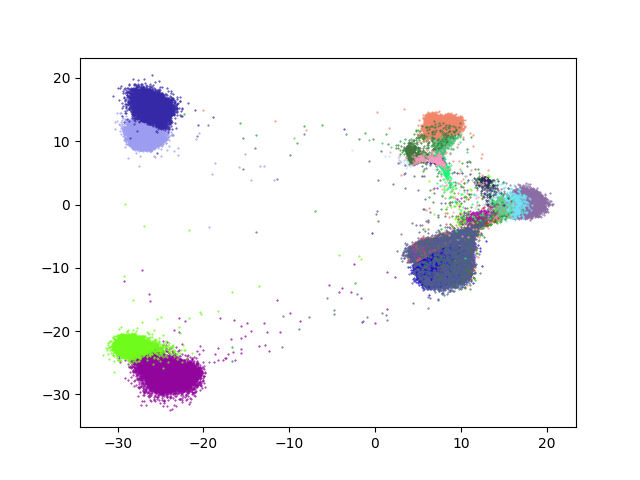
\includegraphics[width=0.25\textwidth]{images/ptsne_levine.png}} &
    \raisebox{-.5\height}{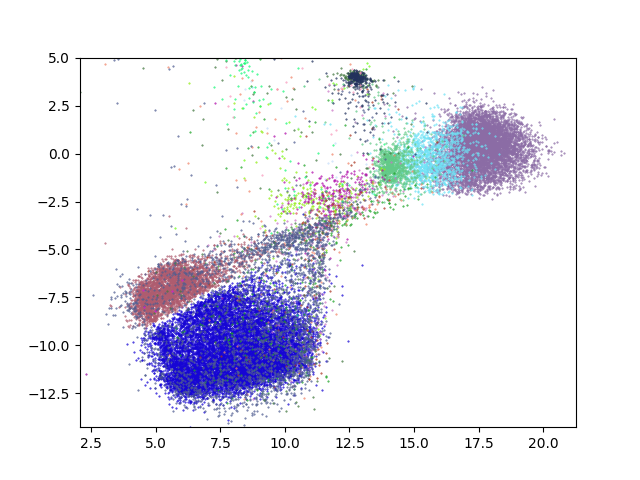
\includegraphics[width=0.25\textwidth]{images/ptsne_levine_zoomed.png}} &
    \raisebox{-.5\height}{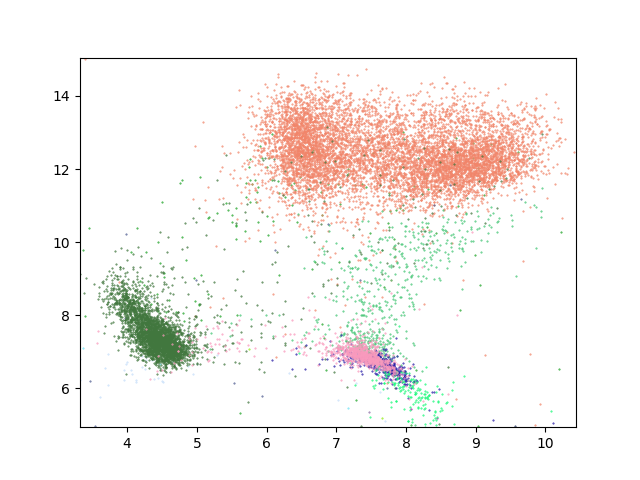
\includegraphics[width=0.25\textwidth]{images/ptsne_levine_zoomed_2.png}} \\
    UMAP &
    \raisebox{-.5\height}{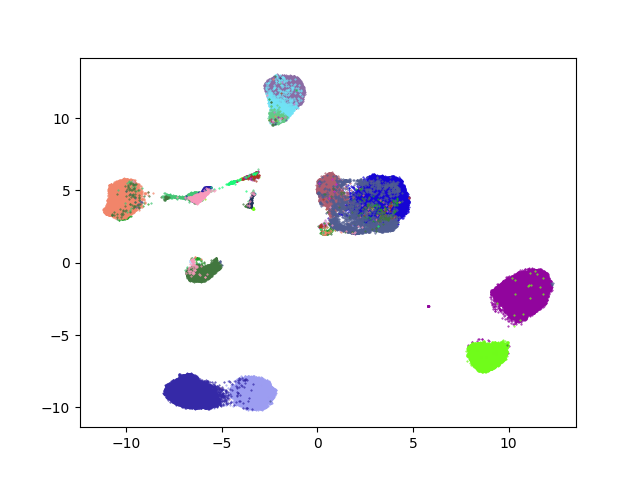
\includegraphics[width=0.25\textwidth]{images/umap_levine.png}} &
    \raisebox{-.5\height}{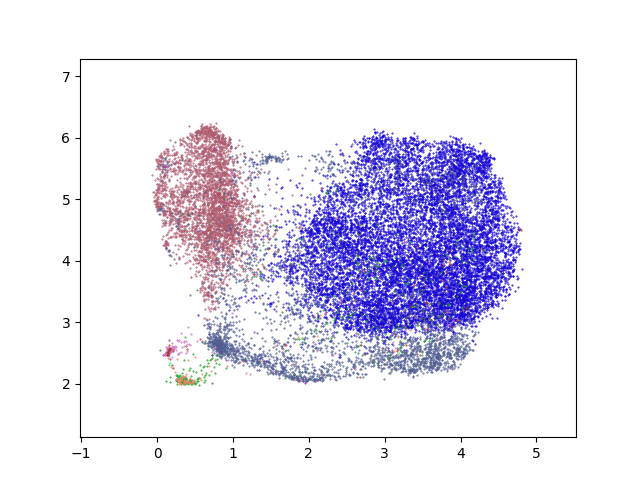
\includegraphics[width=0.25\textwidth]{images/umap_levine_zoomed.png}} &
    \raisebox{-.5\height}{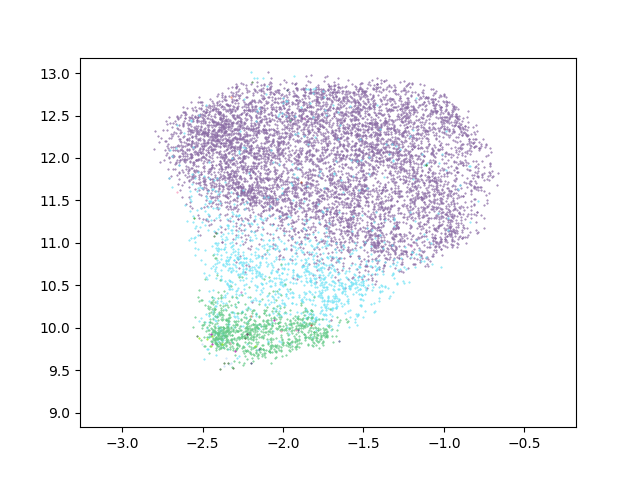
\includegraphics[width=0.25\textwidth]{images/umap_levine_zoomed_2.png}} \\
    VAE &
    \raisebox{-.5\height}{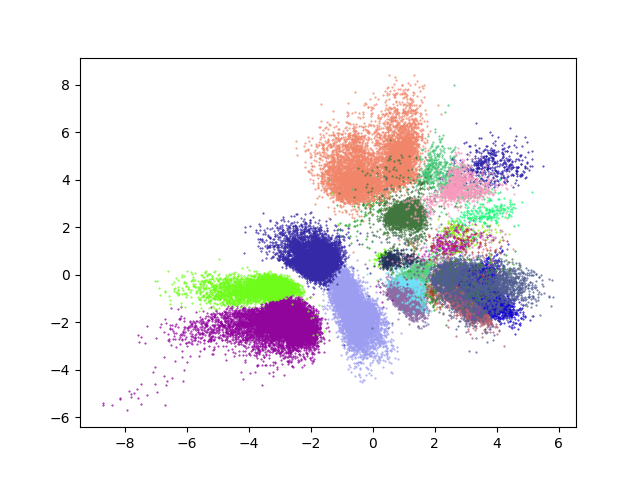
\includegraphics[width=0.25\textwidth]{images/vae_levine.png}} &
    \raisebox{-.5\height}{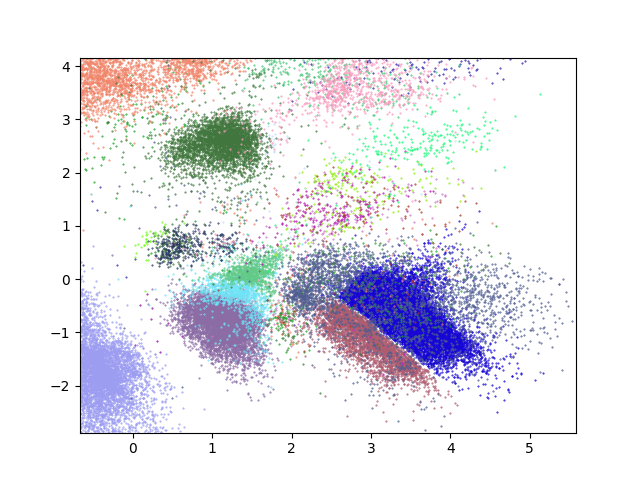
\includegraphics[width=0.25\textwidth]{images/vae_levine_zoomed.png}} &
    \raisebox{-.5\height}{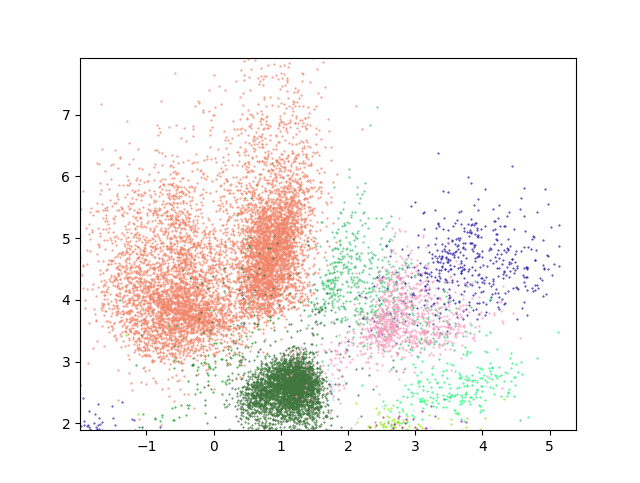
\includegraphics[width=0.25\textwidth]{images/vae_levine_zoomed_2.png}} \\
    t-SNE &
    \raisebox{-.5\height}{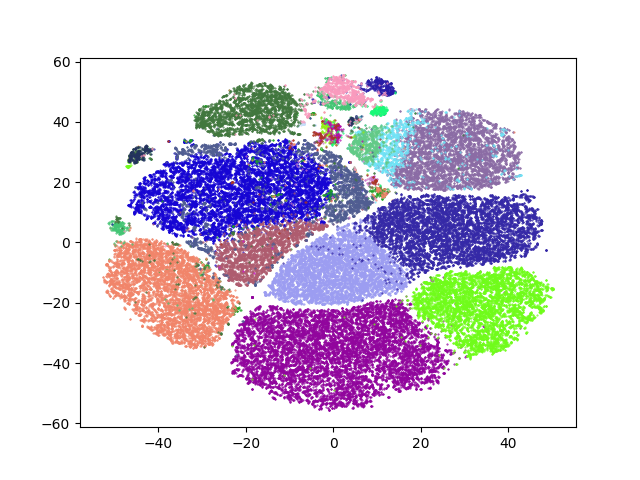
\includegraphics[width=0.25\textwidth]{images/tsne_levine.png}} &
    PCA &
    \raisebox{-.5\height}{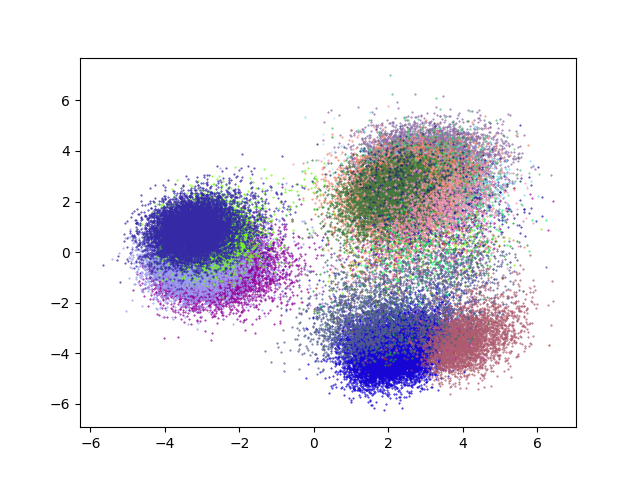
\includegraphics[width=0.25\textwidth]{images/pca_levine.png}} \\
  \end{tabular}
  \caption{Cytometry A data set embedded with the methods being compared in Section~\ref{section:comparisons}.}
  \label{fig:comparison_figure}
\end{figure}

\subsection{Robustness to Sparse Data}

As discussed in Section~\ref{section:robustness} the probabilistic model is advantageous when only few data points are available. To show this effect in practice we trained mappings with and without the use of our method on randomly chosen subsets of the MNIST training data set, effectively simulating sparsity of available training data. Evaluation of the mappings was carried out on the full MNIST test set as in previous experiments. A line plot of the obtained scores corresponding to the chosen size of the subsets can be found in figure \ref{fig:downsampled}. Significant differences in the obtained scores are noted in favor of our method. From these results we can observe that both the trustworthiness and 1-NN scores remain higher even with extremely small data sets, indicating that the use of our method is able to provide better generalization even when few training data points are available.

\begin{figure}[!htb]
  \centering
  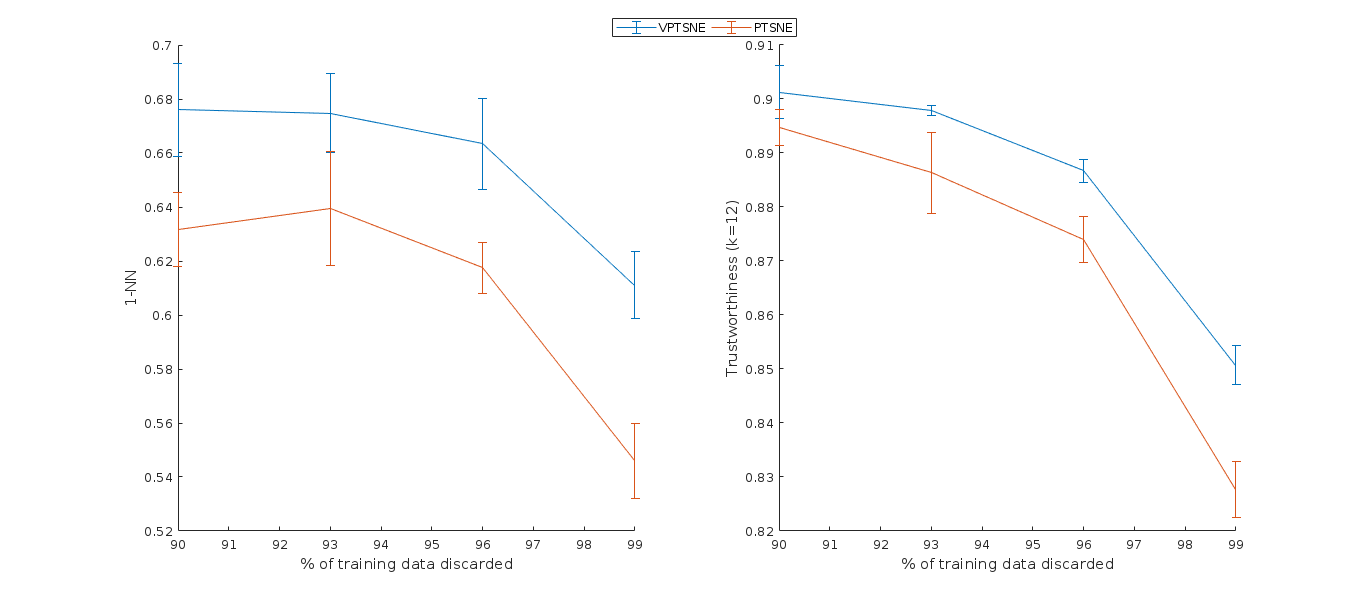
\includegraphics[width=\textwidth]{images/downsampled.png}
  \caption{1-NN and trustworthiness scores obtained for PTSNE and VPTSNE trained on small subsets of the MNIST data set. Error bars indicate the 95\% confidence intervals of the mean for each sparsity level, obtained from 20 repeated runs.}
  \label{fig:downsampled}
\end{figure}

\subsection{Robustness to Noisy Data}

We aim to back up the hypothesis of Section~\ref{section:robustness} by running experiments on artificially corrupted MNIST data sets. As the corruption process in our experiments we consider \textit{masking noise} as in \cite{stacked_denoising_ae}, where a predetermined fraction of randomly chosen elements of a data point are set to 0. We test robustness by applying masking noise to 10\%, 20\%, 30\% and 40\% fractions of the training and test sets. The results of our experiments presented in Figure~\ref{fig:corrupted_data} show a clear advantage to using our method when dealing with noisy data as both evaluation metrics can be observed to decrease considerably for PTSNE as the training data is progressively corrupted, whereas the performance of VPTSNE suffers less throughout the experiments.

As an example of real-world data corrupted in this fashion, in scRNA-seq so-called \textit{dropout events} \cite{sc_dropout}, which cause incomplete sequence data to be captured due to technical and biological noise, can be viewed as a form of masking noise. The results presented here would indicate that the proposed method is potentially a good fit for exploratory analysis of scRNA-seq data, even without attempting to explicitly correct for the present technical noise, as in e.g. \cite{zifa} where factor analysis is extended to additionally model dropouts.

Even with the standard VAE structure, the obtained results are encouraging. As future work it would be interesting to test whether making use of denoising variational autoencoders \cite{denoising_vae}, which are an extension of denoising autoencoders \cite{stacked_denoising_ae} that are directly trained to correct corrupted data. Additionally of interest is how our method fares when other corruption processes are present.

\begin{figure}[!htb]
  \centering
  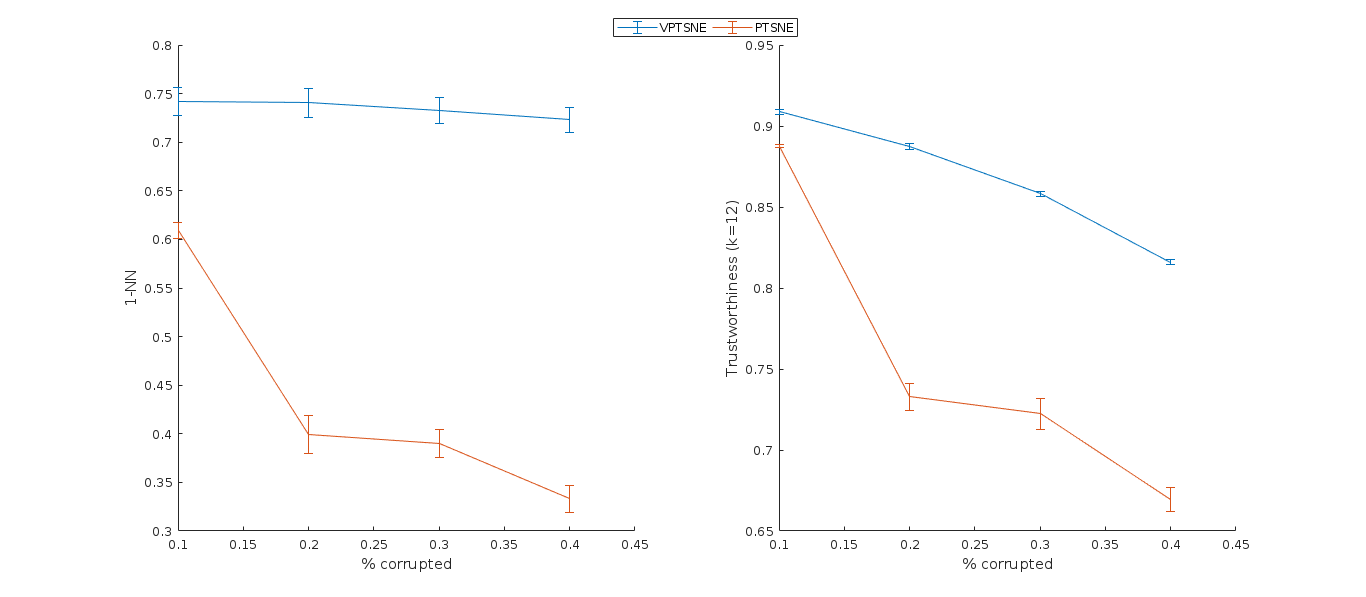
\includegraphics[width=\textwidth]{images/corrupted.png}
  \caption{1-NN and trustworthiness scores obtained for PTSNE and VPTSNE trained on MNIST data with different levels of masking noise applied. Error bars indicate the 95\% confidence intervals of the mean for each corruption level, obtained from 20 repeated runs.}
  \label{fig:corrupted_data}
\end{figure}

\subsection{Obtaining Reconstructions from Hidden Layers}

To show the efficacy of this modification to the learning procedure we train an embedding using the latent code directly. As we choose the dimensionality of the latent code to be more than two orders of magnitude smaller than that of the original data's it is possible for us to use batches of greater size to train the embedding network, without incurring additional computation cost over training with smaller batches on data of the original dimensionality. The latent dimensionality of the VAE was chosen to be $7$ and the batch size for training the embedding was set to $5000$, as in the original work on parametric t-SNE \cite{parametric_tsne}. The choice of $7$ as the VAE latent dimensionality was deliberately made so that it would correspond to the largest number which is two orders of magnitude smaller than the original dimensionality. We have additionally included the embedding of data points obtained with the original implementation of parametric t-SNE for comparison in figure \ref{fig:hidden_layer}. Qualitatively and quantitatively an overall better embedding is achieved with less computation using our method.

\begin{figure}[!htb]
  \centering
  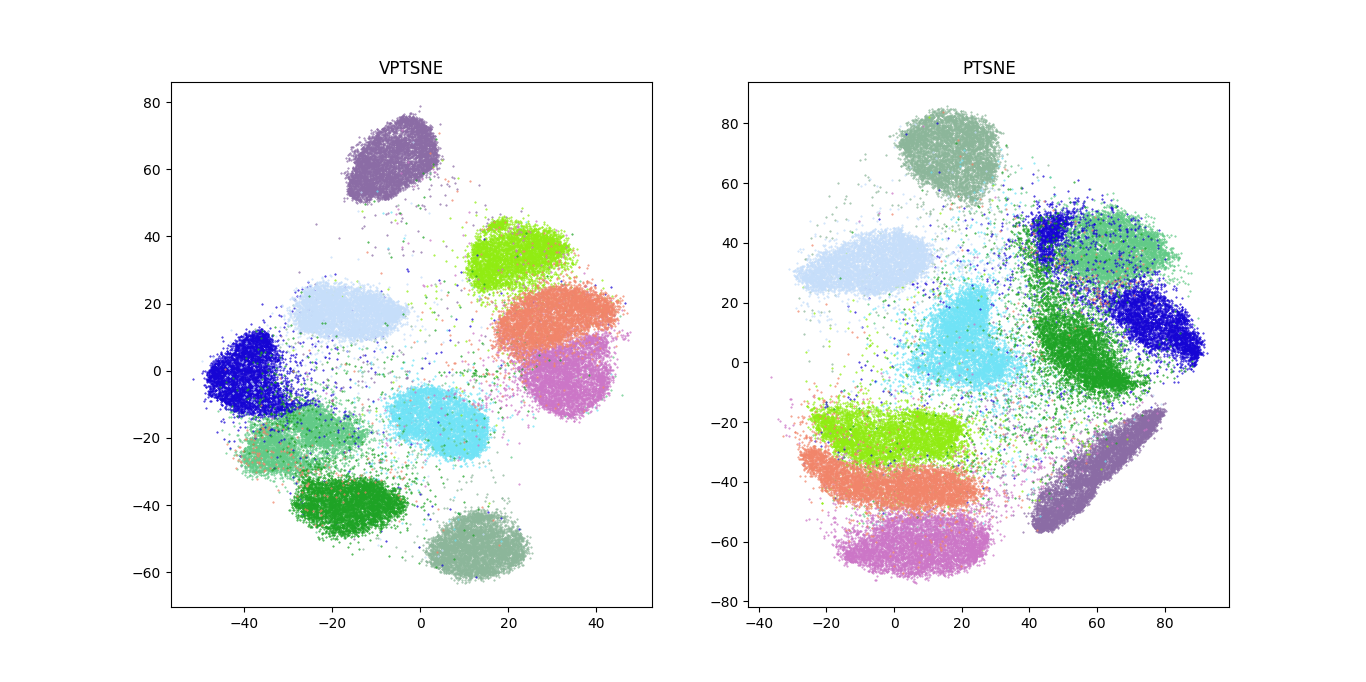
\includegraphics[width=\textwidth]{images/vptsne_vs_original_ptsne_7.png}
  \caption{Embedding produced by training on a 7 dimensional latent representation of the MNIST data set contrasted with the result of the original PTSNE implementation. VPTSNE trustworthiness: 0.927, 1-NN: 0.910. PTSNE trustworthiness: 0.926, 1-NN 0.887.}
  \label{fig:hidden_layer}
\end{figure}

\section{Application to Single-Cell Data Analysis}
\label{section:applications}

\subsection{Inference with the Generative Model}
\label{section:application_inference_with_the_generative_model}

As an example of inference with the generative model discussed in \ref{section:inference_with_the_generative_model} we use the Cytometry B data set to train our combined model with two patients' data held out. The protein expression profile of Patient A's cells closely match that of other patients' in the training set, whereas Patient B's sample is from advanced cancer making it an outlier in relation to the data available during training. As these cells feature a distinct phenotype associated with a poor response to treatment, they might confer resistance to chemotherapy.

To distinguish between outlier and inlier points in the obtained mapping we set a hard threshold of $\log p(\bx) < -150$ to separate between the two. In figure \ref{fig:cytometry_outliers} embeddings with both patient specific labeling and labeling obtained by thresholding are shown side by side. The high tumor purity sample of Patient B has almost completely been mapped to a small region corresponding to protein expression levels of cancer cells, whereas Patient A's mapping contains several distinct clusters of various cell types. Further, the labels obtained through thresholding indicate that the majority of cells in Patient B's sample are indeed considered as outliers by the model, in addition to a handful of visually poorly mapped points.

\begin{figure}[!htb]
  \centering
  \begin{tabular}{c}
    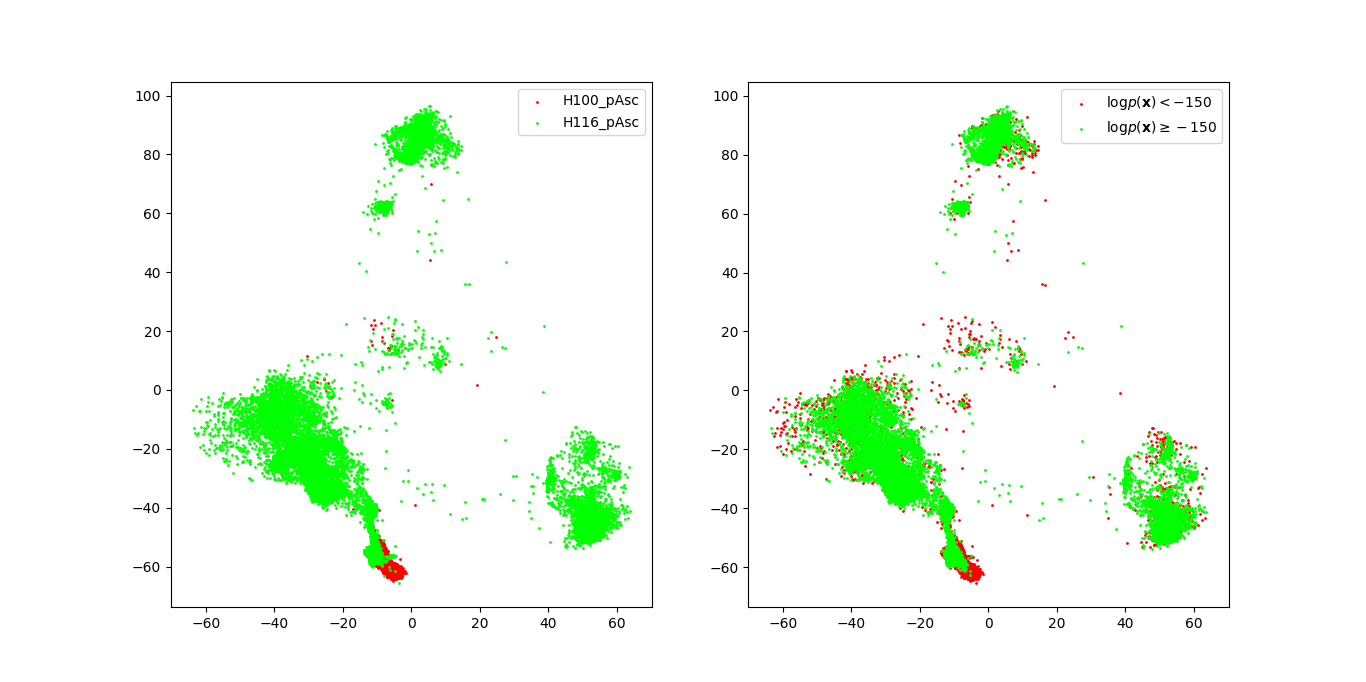
\includegraphics[width=\textwidth]{images/scored.png} \\
    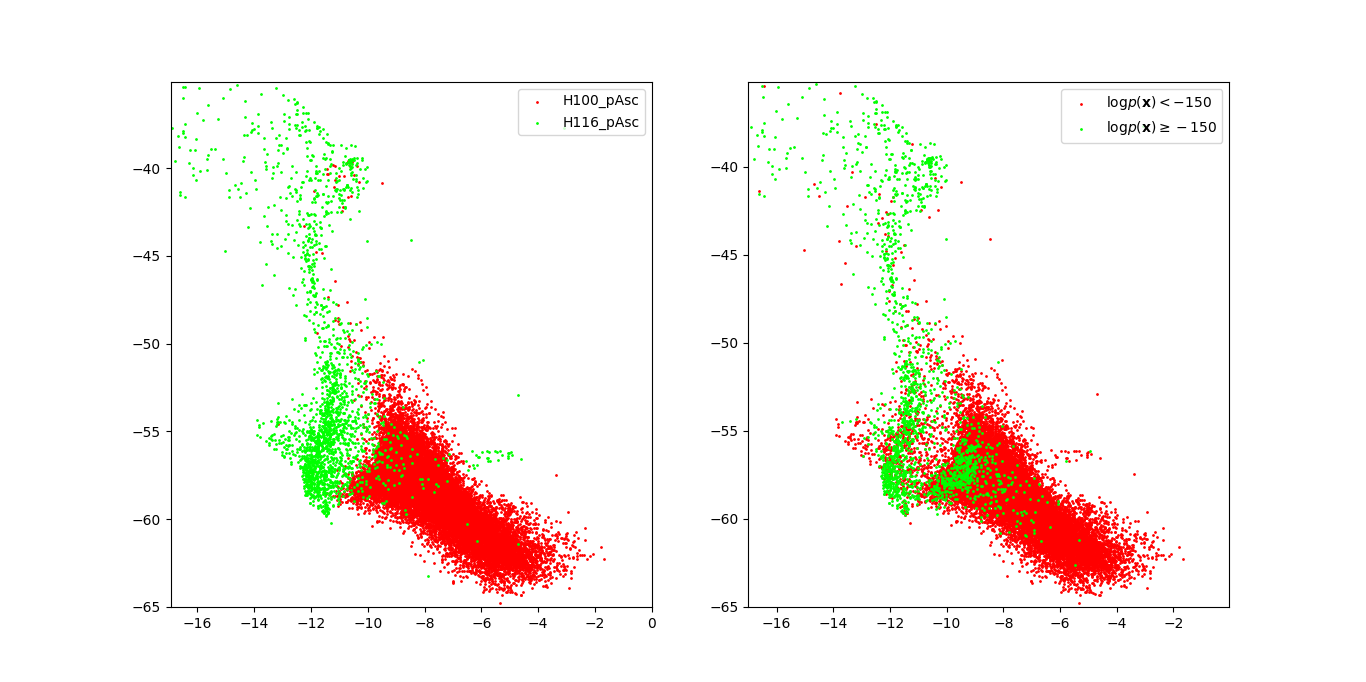
\includegraphics[width=\textwidth]{images/scored_zoomed.png}
  \end{tabular}
  \caption{Detecting outliers in cytometry data.}
  \label{fig:cytometry_outliers}
\end{figure}

\subsection{Application to scRNA-seq Data}
\label{section:application_to_scrna}

Noting the results presented in the previous sections, we finally aim to demonstrate the applicability of our method to a real-world data set that is both sparse and very high dimensional, as well as contains corruption due to technical variation. For this purpose the scRNA-seq data set of \cite{tirosh} was chosen.

Due to the very high dimensionality in comparison to the other data sets, more capacity to the VAE network was added. The layer dimensions for the VAE architecture were chosen to be $d - 1000 - 1000 - 500 - \mu, \log \sigma^2 - 500 - 1000 - 1000 - d$ and $50$ was chosen as the latent dimensionality. To train the embedding we used the method of obtaining the reconstructed data points directly from the latent code.

In Figure~\ref{fig:tirosh} we have visualized the data of \cite{tirosh} using our method and the results of the analysis carried out in the study.

From the results we can see that different tumor samples and cell types cluster well in the embedding. The separation of malignant cells from different patients to separate clusters reveals the heterogeneity of melanoma present in the different tumor samples.

For each cell in the data set so-called MITF- and AXL-program scores were computed from the relative expression levels of their corresponding gene sets, as in \cite{tirosh}. These scores aim to provide insight into the potential drug resistance mechanisms of malignant cells \cite{mitf, mitf_axl}. In our embedding a clear gradient from high to low MITF- and AXL-program scores can be seen within the cluster of tumor cell clusters, further indicating that our method is able to highlight biologically meaningful variations in the data.

Cell cycle analysis also reveals the presence of subclusters of cycling cells in our embedding. Cycling cells being cells which are undergoing cell division. The color gradient in the projection for cycling cells corresponds to the strength of the signal indicating cell cycling. Below a given threshold value for this signal, cells were classified as non-cycling.

With such a high dimensional data set, the effect of the curse of dimensionality can be seen on methods based on distances, leading them to produce inferior embeddings. For example, applying UMAP directly to the high dimensional data, a couple of the most obvious shortcomings of the embedding is its failure to distinguish between different cell types as well as being unable to properly separate tumor cell clusters originating from different samples. A figure of the UMAP embedding is included in Appendix~\ref{appendix:umap_tirosh} for comparison.

\begin{figure}[!htb]
  \centering
  \begin{tabular}{cc}
    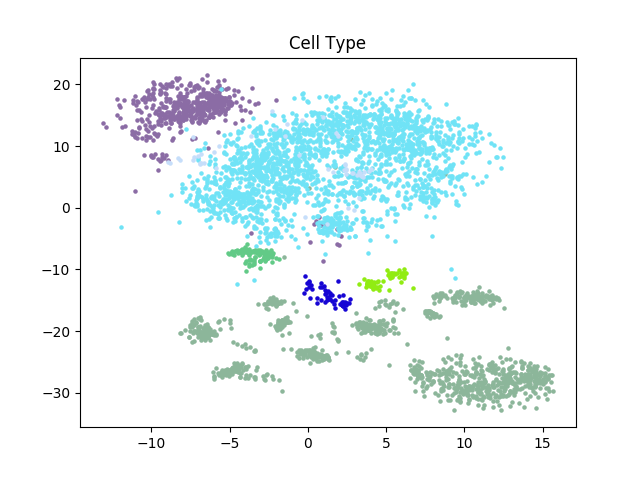
\includegraphics[width=0.5\textwidth]{images/tvptsne_cell.png} &
    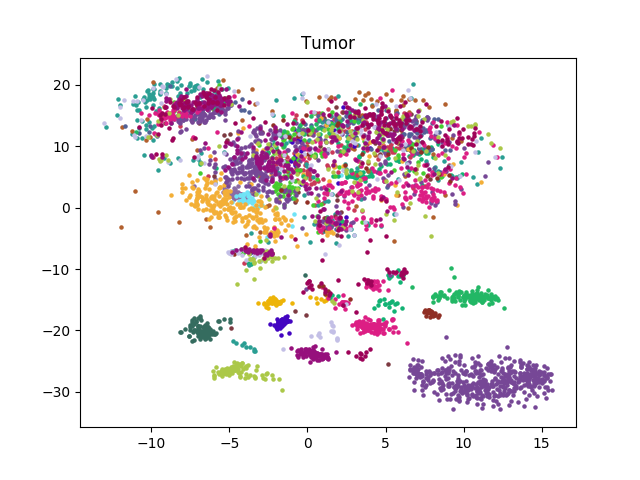
\includegraphics[width=0.5\textwidth]{images/tvptsne_tumor.png} \\
    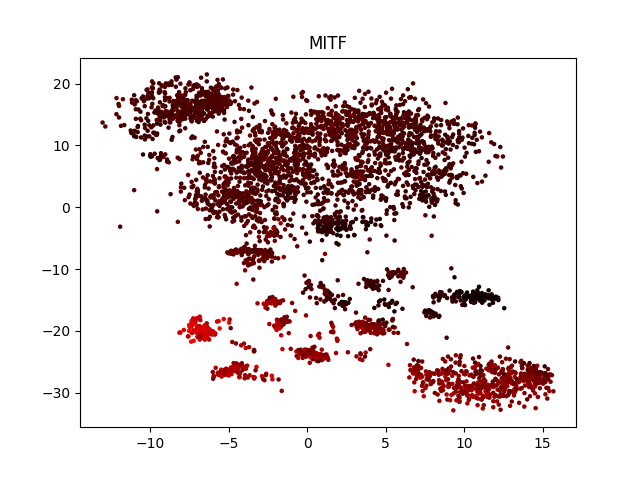
\includegraphics[width=0.5\textwidth]{images/tvptsne_mitf.png} &
    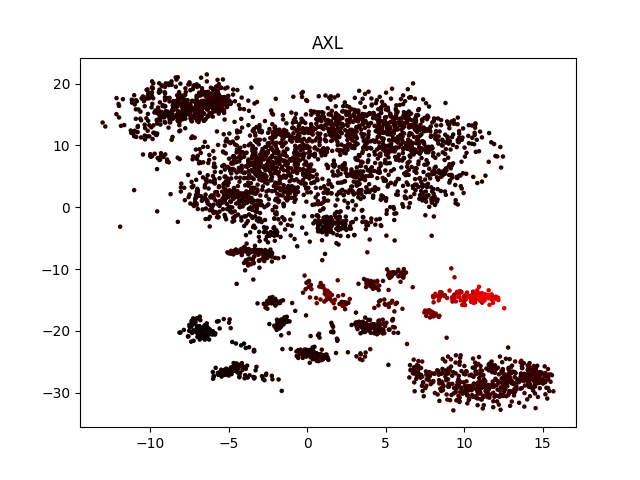
\includegraphics[width=0.5\textwidth]{images/tvptsne_axl.png} \\
    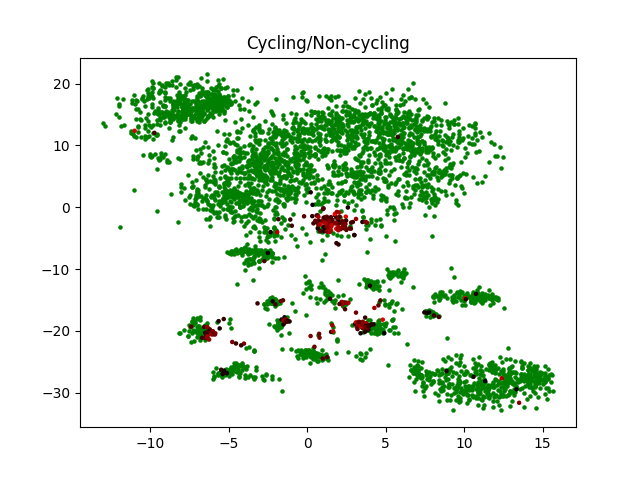
\includegraphics[width=0.5\textwidth]{images/tvptsne_cycling.png} &
    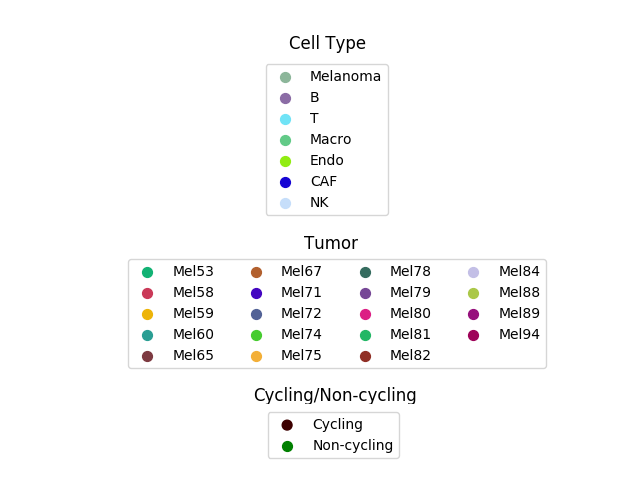
\includegraphics[width=0.5\textwidth]{images/tirosh_all_legends.png} \\
  \end{tabular}
  \caption{Visualization of analysis results on data from \cite{tirosh} using VPTSNE.}
  \label{fig:tirosh}
\end{figure}

\chapter{Conclusions}
\label{ch:conclusions}

By combining two dimensionality reduction methods: a stochastic variant of autoencoders and a neural network parameterized variant of t-SNE, we demonstrated a method for parametric dimensionality reduction exhibiting various advantageous properties in comparison to either method applied by itself. \note{.. recap results ..}

In addition, two applications of the method to single-cell data analysis were demonstrated in this work. The method was applied to both moderately high dimensional proteomic data and extremely high dimensional transcriptomic data. \note{.. recap more results ..}

\note{.. Why development of new methods is important [to better analyze ever more complex data, gathered with continuously developing technology] ..}

\note{.. Future work ..}

\ifnameyear
  \bibliographystyle{babapaliktutnat}
\else
  \bibliographystyle{bababbrtut}
\fi
\bibliography{main}

\appendix
\chapter{Small Batch Size, Low Perplexity Embedding}
\label{appendix:low_perp_small_bs}
\begin{figure}[!htb]
  \centering
  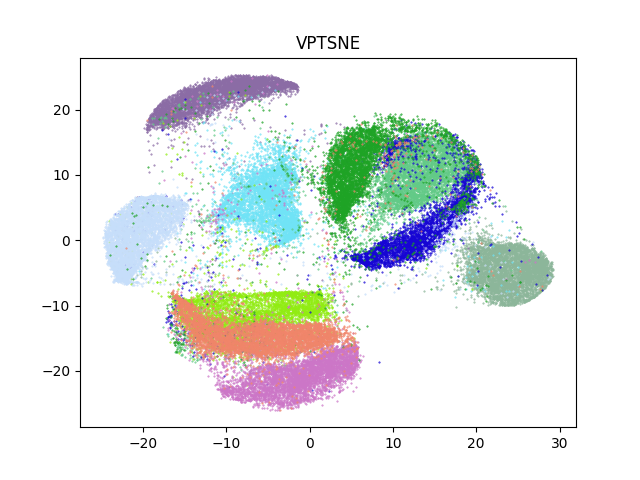
\includegraphics[width=\textwidth]{images/mnist_vptsne_bs_200_perp_10.png} 
  \caption{Effect of the choice of perplexity w.r.t. batch size. MNIST VPTSNE embedding trained with batch size 200 and perplexity 10. Trustworthiness: 0.935, 1-NN: 0.812.}
  \label{fig:low_perp_small_bs}
\end{figure}

\chapter{UMAP Embedding of scRNA-seq Data}
\label{appendix:umap_tirosh}
\begin{figure}[!htb]
  \centering
  \begin{tabular}{cc}
    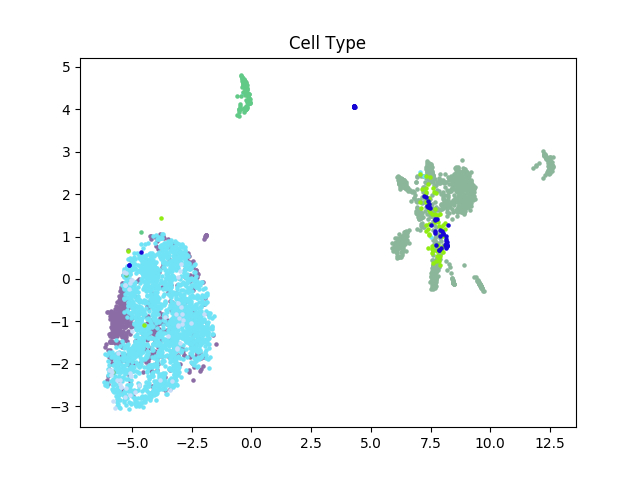
\includegraphics[width=0.5\textwidth]{images/tumap_cell.png} &
    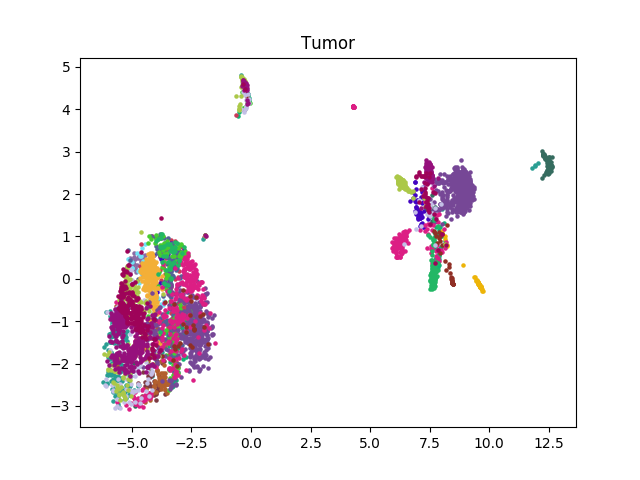
\includegraphics[width=0.5\textwidth]{images/tumap_tumor.png} \\
    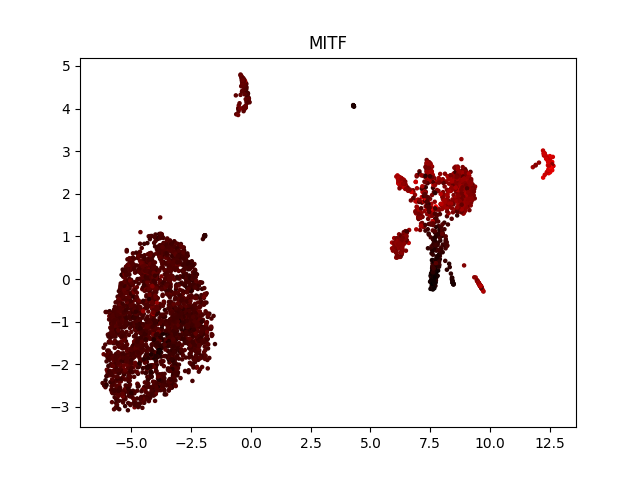
\includegraphics[width=0.5\textwidth]{images/tumap_mitf.png} &
    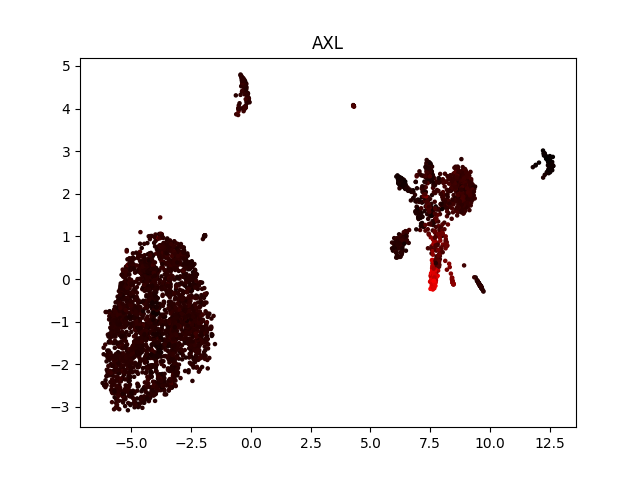
\includegraphics[width=0.5\textwidth]{images/tumap_axl.png} \\
    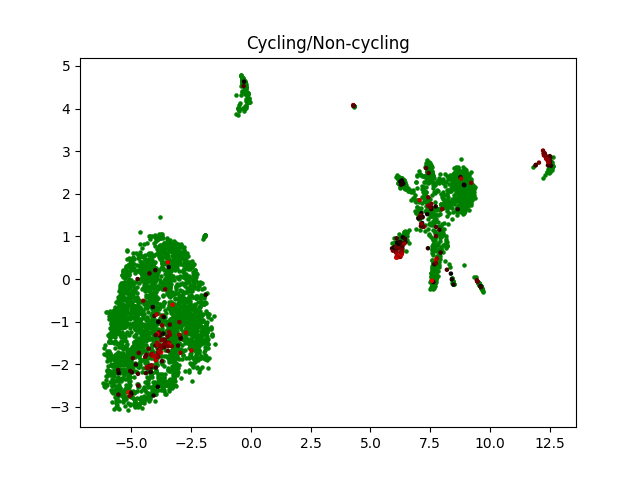
\includegraphics[width=0.5\textwidth]{images/tumap_cycling.png} &
    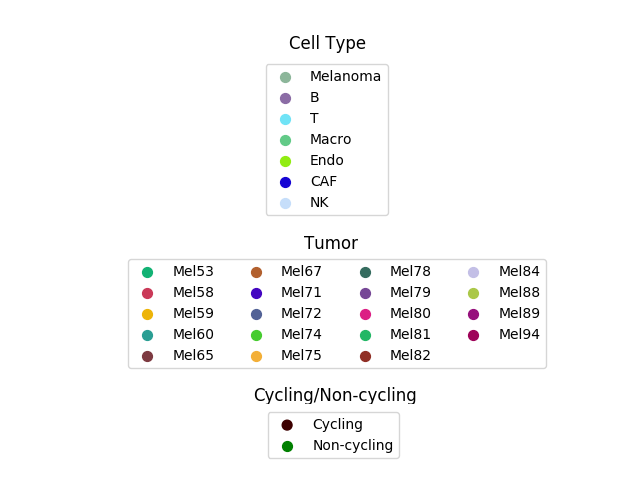
\includegraphics[width=0.5\textwidth]{images/tirosh_all_legends.png} \\
  \end{tabular}
  \caption{Visualization of analysis results on data from \cite{tirosh} using UMAP.}
  \label{fig:tirosh_umap}
\end{figure}

